\documentclass[oneside,fontsize=11pt,paper=a4]{scrartcl}
\usepackage[margin=1.5cm]{geometry}
\usepackage[utf8]{inputenc}
\usepackage[english]{babel}
\usepackage[autostyle]{csquotes}
\usepackage{url}
\usepackage{hyperref}
\usepackage{siunitx}
\usepackage{hyperref}
\usepackage{amsfonts}
\usepackage{amsmath}
\usepackage{amssymb}
\usepackage{multicol}
\usepackage{enumitem}
\usepackage{graphicx}
\usepackage{mathtools}
\usepackage{bm}
\usepackage{url}
\usepackage{xcolor}
\usepackage{soul}
\usepackage{tabularx}
\usepackage{makecell}

\geometry{footskip=1cm}

\urlstyle{same}
\setlength\parindent{0pt}
\setlist[description]{font=\normalfont\bfseries, style=unboxed}

\newcommand{\A}[5]{\left#1\begin{array}{ccc}
{#2}_{11}B & \cdots & {#2}_{1#4}B\\
\vdots & \ddots & \vdots\\
{#2}_{#31}B & \cdots & {#2}_{#3#4}B
\end{array}\right#5}

\newcommand{\hlc}[2][yellow]{ {\sethlcolor{#1} \hl{#2}} }
\newcommand{\mathcolorbox}[2]{\colorbox{#1}{$\displaystyle #2$}}
\newcommand*{\Scale}[2][4]{\scalebox{#1}{$#2$}}%

\newcolumntype{Y}{>{\centering\arraybackslash}X}

\newenvironment{myfigure}
  {\par\medskip\noindent\minipage{\linewidth}}
  {\endminipage\par\medskip}

\title{Computer Vision 2 - Multiple View Geometry Class (IN2228): Summary}
\author{Franz Kaschner \\ Technical University of Munich \\}
\date{Summer Semester 2022}

\begin{document}
\maketitle

\begin{abstract}
\noindent This document summarizes the main topics and key aspects of the lecture ''Computer Vision 2 - Multiple View Geometry``. The structure follows the script by Prof. Daniel Cremers. However, for better understanding some content from linear algebra is added. The summary builds on the summary by Marcel Brucker.
\end{abstract}

\begin{multicols}{2}[\section{Mathematical Background: Linear Algebra}]
\subsection{Set}
A Set $S$ of different elements e.g. the Natural numbers $\mathbb{N} = \{1, 2, 3, \dots\}$ or the set of all real $n \times n$- matrices $\mathcal{M}(n)$.

\subsection{Vector Space}
A set $V$ is called a vector space over the field $\mathbb{R}$ if it is closed under vector summation
\begin{equation*}
	+: V \times V \rightarrow V
\end{equation*}
and under scalar multiplication
\begin{equation*}
	\cdot: \mathbb{R} \times V \rightarrow V
\end{equation*}

\subsection{Linear Transformations}
A linear transformation L between two linear spaces V and W is a map $L: V \rightarrow W$ such that:
\begin{itemize}
    \item $L(x+y)=L(x)+L(y), \forall x,y \in V$
    \item $L(\alpha x) = \alpha L(x), \forall x \in V, \alpha \in \mathbb{R} $
\end{itemize}

\subsection{Linear Independence}
A set of vectors $S = \{v_1, \dots, v_k \} \subset V$ is the subspace formed by all linear combinations of these vectors:
\begin{equation*}
	\text{span}(S) = \left\{ v \in V \,\middle\vert\, v = \sum_{i=1}^k \alpha_i v_i \right\}
\end{equation*}
Linear independence holds if none of the vectors can be expressed as a linear combination of the remaining vectors.\\
In $\mathbb{R}^3$ for instance, row reduce the matrix
\begin{equation*}
	S = \begin{pmatrix} v_{1x} &  v_{1y} & v_{1z}\\  v_{2x} & v_{2y} & v_{2z} \\ v_{3x} & v_{3y} & v_{3z} \end{pmatrix}
\end{equation*}
using Gauss-Jordan elimination.
If you can make one row all zeroes, then your set is linearly dependent (since one row is a multiple of the other).
Alternatively, check if the determinant 
\begin{equation*}
	\det(S) = 0
\end{equation*}
is zero. If so, $v_1$, $v_2$ and $v_3$ are linearly independent.\\
Linear dependence for a set of vectors $v_i$ holds if
\begin{equation*}
	\sum_{i=1}^{n} \alpha_i v_i = 0 \quad \alpha_i \in \mathbb{R} \ \text{(not all zero)}, v_i \in \mathbb{R}^n
\end{equation*}

\subsection{Basis}
A set of vectors $B = {v_1, \dots, v_n}$ is called a basis of $V$ if it is linearly independent and if it spans the vector space $V$. A basis is a maximal set of linearly independent vectors. Properties ($B$ and $B'$ are two bases of a linear space $V$):
\begin{itemize}
	\item $B$ and $B'$ contain the same number of vectors, which is called the dimension of the space $V$.
	\item Any vector can be uniquely expressed as a linear combination of the basis vectors.
	\item All vectors can be expressed as linear combination of vectors of another basis.
\end{itemize}

\subsection{Dot Product}
\begin{equation*}
	\langle \cdot, \cdot \rangle: V \times V \rightarrow \mathbb{R}
\end{equation*}
Two vectors $v$ and $w$ are orthogonal iff $\langle v, w \rangle = 0$. \\

Properties:
\begin{itemize}
	\item $\langle u, \alpha v + \beta w \rangle = \alpha \langle u,w \rangle + \beta \langle u,w \rangle$ (linear)
	\item $\langle u,v \rangle = \langle v,u \rangle$ (symmetric)
	\item $\langle v, v \rangle \geq 0 $ and $ \langle v,v \rangle = 0 \iff v = 0$ (positive definite)
\end{itemize}
Canonical inner product: $\langle u,v \rangle = u^T v$

%\subsection{Norms \& metrics}

\subsection{Kronecker Product and stack}
Given two matrices $A \in \mathbb{R}^{m \times n}$, $B \in \mathbb{R}^{k \times l}$, one can define their Kronecker product $A \otimes B$ by:
\begin{flalign*}
	A \otimes B \equiv& \A(amn) \in \mathbb{R}^{mk \times nl} \\
	&(A \otimes B)^T = A^T \otimes B^T
\end{flalign*}

Given a matrix $A \in \mathbb{R}^{m \times n}$, its stack $A^S$ is obtained by stacking its $n$ column vectors $a_1, ..., a_n \in \mathbb{R}^{m}$:
\begin{equation*}
	A^S \equiv 
	\begin{pmatrix}
		a_1 \\
		\vdots \\
		a_n \\
	\end{pmatrix}	
	\in \mathbb{R}^{mn}
\end{equation*}

\begin{equation*}
	u^T A v = (v \otimes u)^T A^S
\end{equation*}
\begin{equation*}
	(A \otimes B)^T = A^T \otimes B^T
\end{equation*}

\subsection{Group}
A set $S$ combined with a defined operation $\circ$, e.g. ($\mathbb{N}$, $\cdot$), with properties:
\begin{enumerate}
	\item $a \circ b \in S$ (closed)
	\item $(a \circ b) \circ c = a \circ (b \circ c)$ (associative)
	\item $a \circ n = a$ ($n$ is a neutral element in S)
	\item $a \circ a^{-1} = n$ (every element has an inverse element)
\end{enumerate}
(Abelian groups are commutative in addition: $a \circ b = b \circ a$.)

\subsection{Ring}
A set $S$ combined with two defined operations and properties from above, e.g. ($\mathbb{N}$, $+$, $\cdot$).

\subsection{Field}
A ring which is distributive in addition: $a \cdot (b + c) = a \cdot b + a \cdot c$, e.g. ($\mathbb{R}$, $+$, $\cdot$).

\subsection{Popular Groups}
\begin{itemize}
    \item General linear group:\\
    $GL(n) = (\{A \in \mathbb{R}^{n \times n} \; \vert \; \det(A) \neq 0\}, \; \cdot \;)$\\
    Operation: matrix multiplication.
    \item Special linear group:\\
    $SL(n) = \{A \in GL(n) \; \vert \; \det(A) = +1\}$
    \item Orthogonal group:\\
    $O(n) = \left\{ R \in GL(n) \; \vert \; R^TR = RR^T = I \right\}$\\
    Set of all orthogonal matrices ($\det R = \pm1$).
    \item Special orthogonal group:\\
    $SO(n) = \{A \in O(n) \; \vert \; \det(A) = +1\}$\\
    Rotation matrices, see appendix \ref{section:rotation_matrices}.
    \item Affine group:\\
    $A(n) = \{\begin{psmallmatrix} A & b\\ 0 & 1\\ \end{psmallmatrix} \; \vert \; A \in GL(n), b \in \mathbb{R}^n\}$\\
    Set of all affine transformations $L(x) = Ax + b$.
	$\begin{psmallmatrix}
		A & b\\
		0 & 1\\
	\end{psmallmatrix}
	\in GL(n+1)$
    \item Euclidean group:\\
    $E(n) = \{\begin{psmallmatrix} R & T\\ 0 & 1\\ \end{psmallmatrix} \; \vert \; R \in O(n), T \in \mathbb{R}^n\}$\\
    Subgroup of affine group with $L(x) = Rx + T$.
    \item Special Euclidean group:\\
    $SE(n) = \{\begin{psmallmatrix} R & T\\ 0 & 1\\ \end{psmallmatrix} \; \vert \; R \in SO(n), T \in \mathbb{R}^n\}$\\
    Subgroup of $E(n)$. Represents rigid-body motions. $L(x) = Rx + T$.
\end{itemize}
$ SO(n) \subset O(n) \subset GL(n)$ \\
$SE(n) \subset E(n) \subset A(n) \subset GL(n+1)$

\subsection{Subgroup test}
Suppose that $G$ is a group, and $H$ is a subset of $G$. \\
Then $H$ is a subgroup of $G$ if and only if $H$ is nonempty and closed under $\circ$ and inverses. \\
Combination of these two conditions: For every $a$ and $b$ in $H$, the element $a \circ b^{-1}$ is in $H$.

\subsection{Range/Span}
The range of a matrix $A$ is given by the span of its column vectors:
\begin{equation*}
\text{range}(A) = \{ y \in \mathbb{R}^m \ \vert \ \exists x \in \mathbb{R}^n: Ax=y \}
\end{equation*}

\subsection{Kernel/Null Space}
The null space or kernel of a matrix $A$ is given by the subset of vectors $x \in \mathbb{R}^n$ which are mapped to zero:
\begin{equation*}
    \text{null}(A) \equiv \text{ker}(A) = \{x \in \mathbb{R} \mid Ax = 0 \}
\end{equation*}

The LGS $A x = b$ has a solution iff:
\begin{itemize}
    \item $b \in \text{range}(A)$
    \item $\text{ker}(A) = 0 \rightarrow \text{unique solution}$ 
\end{itemize}
$\det(A) \neq 0 \Leftrightarrow \text{rank}(A) = n \Leftrightarrow \text{kernel}(A) = \{0\}$

\subsection{Rank}
The rank of a matrix is the dimension of its range:
\begin{equation*}
    \text{rank}(A) = \text{dim}(\text{range}(A))
\end{equation*}
Properties of the rank of a matrix $A \in \mathbb{R}^{m \times n}$:
\begin{enumerate}
    \item $\text{rank}(A) = n - \text{dim}(\text{ker}(A))$
    \item $0 \leq \text{rank}(A) \leq \min\{m, n\}$
    \item $\text{rank}(A)$ is equal to the maximum number of linearly independent row or column vectors of $A$.
    \item Sylverster's inequality (for $B \in \mathbb{R}^{n \times n}$): $\text{rank}(A) + \text{rank}(B) - n \leq \text{rank}(AB) \leq \min\{\text{rank}(A), \text{rank}(B)\}$
    \item For any invertible matrices $C \in \mathbb{R}^{m \times m}$ and $D \in \mathbb{R}^{n \times n}$, we have: $\text{rank}(A) = \text{rank}(CAD)$.
\end{enumerate}

\subsection{Eigenvalues and Eigenvectors}
Let $A \in \mathbb{C}^{n \times n}$ be a complex matrix. A non-zero vector $v \in \mathbb{C}^{n}$ is called a (right) eigenvector of $A$ if:
\begin{equation*}
    Av = \lambda v \ \text{with } \lambda \in \mathbb{C}, v \neq 0.
\end{equation*}
Properties:
\begin{enumerate}
    \item The eigenvectors of a matrix $A$ associated with different eigenvalues are linearly independent - $\lambda_a \neq \lambda_b \Rightarrow$ $v_a$ and $v_b$ are linearly independent
    \item All eigenvalues $\sigma (A)$ are the roots of the characteristic polynomial $\det(\lambda I-A) = 0$.
    \item If $B = PAP^{-1}$ for some non-singular matrix $P$, then $\sigma (B) = \sigma (A)$.
    \item $\sigma (A) = \sigma (A^T)$.
    \item $A$ is symmetric and PD (or $U = V$) $\Rightarrow$ Eigendecomposition and SVD are equivalent.
\end{enumerate}
Eigendecomposition: $A, V, \Lambda \in \mathbb{R}^{n \times n}$
\begin{equation*}
	A = V \Lambda V^{-1}, \ \Lambda = \text{diag}(\lambda_1, ..., \lambda_n),\
	V =
	\begin{psmallmatrix}
		\vert &  & \vert \\
		v_1 & \cdots  & v_n \\
		\vert &  & \vert \\
	\end{psmallmatrix}
\end{equation*}

\subsection{Symmetric Matrices}
A matrix $S \in \mathbb{R}^{n \times n}$ is called symmetric if $S^T = S$. Properties:
\begin{enumerate}
    \item All eigenvalues of $S$ are real, i.e. $\sigma(S) \subset \mathbb{R}$.
    \item Eigenvectors of $S$ corresponding to distinct eigenvalues are orthogonal.
    \item There always exist $n$ orthonormal eigenvectors of $S$ which form a basis of $\mathbb{R}^3$. $S = V \Lambda V^T$ with $V = (v_1, ..., v_n) \in O(n)$ and $\Lambda = \text{diag}(\lambda_1, ..., \lambda_n)$.
    \item $S$ is PD (PSD), if all eigenvalues are positive (non-negative).
    \item Let $S$ be positive semi-definite and $\lambda_1, \lambda_n$ the largest and smallest eigenvalue. Then $\lambda_1 = \max_{|x|=1} \langle x, Sx \rangle$ and $\lambda_n = \min_{|x|=1} \langle x, Sx \rangle$.
\end{enumerate}

\subsection{Norms}
Induced 2-norm of a matrix $A \in \mathbb{R}^{m \times n}$:
\newcommand\norm[1]{\left\lVert#1\right\rVert}
\begin{equation*}
	\norm{A}_2 = \max_{|x|_2 = 1} \sqrt{\langle x, A^T A x \rangle} = \sigma_1
\end{equation*}
Frobenius norm of $A \in \mathbb{R}^{m \times n}$:
\begin{equation*}
	\norm{A}_F = \sqrt{\sum_{i,j} a_{ij}^2} = \sqrt{\text{Tr}(A^T A)} = \sqrt{\sigma_1^2 + ... + \sigma_n ^2}
\end{equation*}
[$A^T A = V \cdot \text{diag}(\sigma_1^2, ..., \sigma_n^2) \cdot V^T$ with $\sigma_1^2 \geq \sigma_i^2 \geq 0$.]

\subsection{Skew-symmetric Matrices}
A matrix $A \in \mathbb{R}^{n \times n} $ is called skew-symmetric if $A^T = -A$ (equivalent to: $A_{ii} = 0$ and $A_{ij} = - A_{ji}$).
\begin{itemize}
    \item All eigenvalues of $A$ are either zero or purely imaginary.
    \item There exists an orthogonal matrix V such that $A = V \Lambda V^T$ where $\Lambda$ is a block-diagonal matrix.
    \item The rank of any skew-symmetric matrix is even.
\end{itemize}

\subsection{Singular Value Decomposition (SVD)}
\textbf{(Compact SVD)} Let $A \in \mathbb{R}^{m \times n}$ be a matrix
\begin{equation*}
    A = U \Sigma V^T
\end{equation*}
with $p = \text{rank}(A) \leq \min(m,n)$, $U \in \mathbb{R}^{m \times p}$ whose columns are orthonormal ($U^T U = I$), $V \in \mathbb{R}^{n \times p}$ whose columns are orthonormal ($V^T V = I$) and $\Sigma \in \mathbb{R}^{p \times p}, \Sigma = \text{diag}(\sigma_1, ... , \sigma_p)$ with singular values $\sigma_1 \geq ... \geq \sigma_n \geq 0$.
SVD can be seen as a generalization of eigenvalues and eigenvectors to non-square matrices.
The number of non-zero singular values gives us the rank of the matrix $A$.\par
\vspace{3mm}

\textbf{(Full SVD)}
$A = U \Sigma V^T \in \mathbb{R}^{m \times n}$ with orthogonal matrices $U \in \mathbb{R}^{m \times m}$ ($U U^T = U^T U = I$, $\det(U) = \pm 1$) and $V \in \mathbb{R}^{n \times p}$ ($V V^T = V^T V = I$, $\det(V) = \pm 1$).\\
$\Sigma \in \mathbb{R}^{m \times n}$ is a rectangular diagonal matrix with singular values $\Sigma_{ii} = \sigma_i$, $\sigma_1 \geq ... \geq \sigma_n \geq 0$.\par
\vspace{3mm}

\textbf{(Relation to eigenvalue decomposition)}\\
$A^T A = (V \Sigma^T U^T) (U \Sigma V^T) = V \Sigma^T \Sigma V^T$\\
$A A^T = (U \Sigma V^T) (V \Sigma^T U^T) = U \Sigma \Sigma^T U^T$\\
Columns of $V$: Eigenvectors of $A^T A$. \\
Columns of $U$: Eigenvectors of $A A^T$. \\
Non-zero singular values: Square roots of the non-zero eigenvalues of $A^T A$ or $A A^T$.

\subsection{Pseudo Inverse}
Let $A \in \mathbb{R}^{m \times n}$, $V \in \mathbb{R}^{n \times n}$, $\Sigma \in \mathbb{R}^{m \times n}$ and $U \in \mathbb{R}^{m \times m}$.
$\Sigma_1$ is the diagonal matrix of non-zero singular values.
Then:
\begin{equation*}
    A^+ = V \Sigma^+ U^T (= (A^T A)^{-1} A^T) \text{, where } \Sigma^+ = \begin{pmatrix} \Sigma_1^{-1} & 0\\ 0&0\\ \end{pmatrix}
\end{equation*}
$x = A^+ b$ is the least squares solution of $Ax = b$.
\end{multicols}

\newpage

\begin{multicols}{2}[\section{Representing a Moving Scene}]
\subsection{3D Space} \label{subsection:3d_space}
The three-dimensional Euclidean space $\mathbb{E}^3$ consists of all points $p \in \mathbb{E}^3$ characterized by coordinates
\begin{equation*}
    X \equiv (X_1, X_2, X_3)^T \in \mathbb{R}^3.
\end{equation*}
Given two points $X$ and $Y$, one can define a bound vector $v$ as
\begin{equation*}
    v = X - Y \in \mathbb{R}^3.
\end{equation*}

\subsection{Cross product \& skew-symmetric matrices} \label{subsection:cross_product_skew}
On $\mathbb{R}^3$ one can define a cross product
\begin{equation*}
\begin{split}
    \times : \mathbb{R}^3 \times \, \mathbb{R}^3 \rightarrow \mathbb{R}^3: u \times v = \\ \begin{pmatrix} u_2v_3 - u_3v_2\\ u_3v_1 - u_1v_3\\u_1v_2 - u_2v_1 \end{pmatrix} \in \mathbb{R}^3
\end{split}
\end{equation*}
which is a vector orthogonal to $u$ and $v$ ($u \times v = -v \times u$).
The skew-symmetric matrix $\hat{u} \in \mathbb{R}^{3 \times 3}$ replaces the cross product by a matrix multiplication
\begin{equation*}
     u \times v = \hat{u} \cdot v = \begin{pmatrix} 0 & -u_3 & u_2\\ u_3 & 0 & -u_1\\ -u_2 & u_1 & 0 \end{pmatrix} \cdot v.
\end{equation*}
The cross product of a vector with itself equals zero ($u \times u = 0$). A skew-symmetric matrix always has an even rank, so a $3 \times 3$ skew-symmetric matrix has rank $2$ (for $u \neq 0$).

\subsection{Rigid Body Motion}
A rigid body motion is a map
\begin{equation*}
	g_t: \mathbb{R}^3 \rightarrow \mathbb{R}^3; \ X \mapsto g_t(X), \ t \in [0,T]
\end{equation*}
which preserves the norm and inner product (length), the cross product (orientation) and the triple product (volume) of any two vectors.
The rigid body motion can be written as $g_t(x) = Rx + T, \ R \in SO(3), T \in \mathbb{R}^3$.\par

\subsection{The Lie Group SO(3)}
The effect of any infinitesimal rotation $R \in SO(3)$ can be approximated by an element from the space of skew-symmetric matrices $so(3) = \{\hat{w} \, \vert \, w \in \mathbb{R}^3\}$.
The rotation group $SO(3)$ is called a Lie group.
The space $so(3)$ is called its Lie algebra and it is a linear space.\par

\textbf{Definition Lie group:} Smooth manifold that is also a group, s.t. the group operations multiplication and inversions are smooth maps.\\\par

\textbf{Definition Lie algebra:} The tangent space of a Lie group at the identity element is called the associated Lie algebra.\\\par

The matrix exponential defines a map from the Lie algebra to the Lie group
\begin{equation*}
    \exp: so(3) \rightarrow SO(3); \ \hat{w} \mapsto e^{\hat{w}} \; (= R)
\end{equation*}
The inverse of the matrix exponential sets is
\begin{equation*}
    \log: SO(3) \rightarrow so(3); \ R \mapsto \log(R) \; (= \hat{w}).
\end{equation*}
The matrix exponential $e^{\hat{w}} = R$ is calculated through the Rodrigues' formula
\begin{equation*}
    e^{\hat{w}} = I + \frac{\hat{w}}{|w|} \sin(|w|) + \frac{\hat{w}^2}{|w|^2} \left(1-\cos\left(|w|\right)\right)
\end{equation*}
and its inverse for obtaining $w$ through ($R \neq I$)
\begin{equation*}
\begin{split}
   |w| = \cos^{-1} \left(\frac{\text{Tr}(R)-1}{2} \right), \\ \frac{w}{|w|} = \frac{1}{2\sin\left(|w|\right)} \begin{pmatrix}r_{32} - r_{23}\\ r_{13} - r_{31}\\ r_{21} - r_{12} \end{pmatrix}
\end{split}
\end{equation*}
For $w = 0$, we have $e^{\hat{w}} = I$.

Any orthogonal transformation $R \in SO(3)$ (see appendix \ref{section:rotation_matrices}) can be realized by rotating by an angle $|w|$ around
an axis $\frac{w}{|w|}$.

\begin{myfigure}
	\centering
	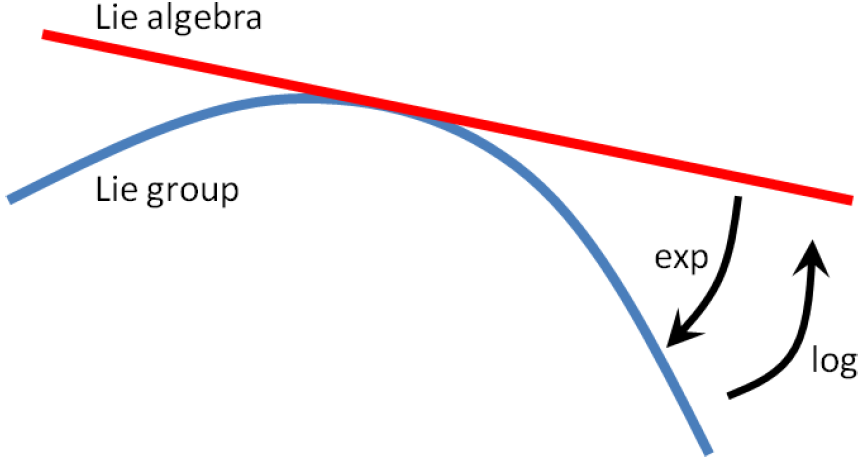
\includegraphics[width=0.6\linewidth]{Images/lie_group_algebra.PNG}
\end{myfigure}

\subsection{The Lie Group SE(3)}
The space of rigid body motions given by the group of special euclidean transformations
\begin{equation*}
    SE(3) \equiv \left\{g = (R, T) \,\middle\vert\, R \in SO(3), T \in \mathbb{R}^3 \right\}.
\end{equation*}
In homogeneous coordinates, we have:
\begin{equation*}
    SE(3) \equiv \left\{g = \begin{psmallmatrix} R & T\\ 0 & 1 \end{psmallmatrix} \,\middle\vert\, R \in SO(3), T \in \mathbb{R}^3 \right\} \subset \mathbb{R}^{4 \times 4}.
\end{equation*}
As in the case of $so(3)$, the set of all twists forms a tangent space which is the Lie algebra
\begin{equation*}
\begin{split}
    se(3) \equiv \left\{\hat{\xi} = \begin{psmallmatrix} \hat{w} & v\\ 0 & 0 \end{psmallmatrix} \,\middle\vert\, \hat{w} \in so(3), v \in \mathbb{R}^3 \right\} \subset \mathbb{R}^{4 \times 4}\\
    \text{with} \quad v(t) = \dot{T}(t) - \hat{w}(t)T(t)
\end{split}
\end{equation*}
to the Lie Group $SE(3)$ ($v$ as linear velocity, $w$ as angular velocity).
Operators $\wedge$ and $\vee$ convert between a twist $\hat{\xi} \in se(3)$ and its twist coordinates $\xi \in \mathbb{R}^6$:
\begin{flalign*}
    \hat{\xi} \equiv \begin{pmatrix} v\\w \end{pmatrix}^{\wedge} &\equiv \begin{pmatrix} \hat{w} & v\\0 & 0 \end{pmatrix} \in \mathbb{R}^{4 \times 4}\\
    \begin{pmatrix} \hat{w} & v\\0 & 0 \end{pmatrix}^{\vee} &= \begin{pmatrix} v\\ w \end{pmatrix} \in \mathbb{R}^6
\end{flalign*}
The exponential map defines a transformation from the Lie Algebra $se(3)$ to the Lie Group $SE(3)$:
\begin{equation*}
	\exp: se(3) \rightarrow SE(3); \ \hat{\xi} \mapsto e^{\hat{\xi}}
\end{equation*}
For $w = 0$, we have $e^{\hat{\xi}} = \begin{pmatrix}I & v\\ 0 & 1 \end{pmatrix}$, and for $w \neq 0$:
\begin{equation*}
    e^{\hat{\xi}} = \begin{pmatrix}e^{\hat{w}} & \frac{(I-e^{\hat{w}})\hat{w}v + ww^Tv}{|w|^2}\\ 0 & 1 \end{pmatrix} = \begin{pmatrix}R & T\\0 & 1 \end{pmatrix} = g
\end{equation*}
For the inverse function and further information see \url{http://ethaneade.com/lie.pdf}.

\subsection{Representing the Camera Motion}
The rigid-body transformation
\begin{equation*}
    g(t) = \begin{pmatrix} R(t) & T(t)\\0 & 1 \end{pmatrix} \in SE(3)
\end{equation*}
represents the motion from a fixed world frame to the camera frame at time $t$.
In particular we assume that at time $t = 0$ the camera frame coincides with the world frame, i.e. $g(0) = I$.
For any point $X_0$ in world coordinates, its coordinates in the camera frame at time $t$ are:
\begin{equation*}
    X(t) = R(t)X_0 + T(t)
\end{equation*}
or in homogeneous representation
\begin{equation*}
    X(t) = g(t)X_0.
\end{equation*}
We denote the transformation from the points in frame $t_1$ to the points in frame $t_2$ by $g(t_2,t_1)$:
\begin{equation*}
    X(t_2) = g(t_2, t_1)X(t_1).
\end{equation*}
\begin{equation*}
    g(t_1, t_2)g(t_2, t_1) = I \Leftrightarrow g^{-1}(t_2, t_1) = g(t_1, t_2)
\end{equation*}
For velocity transformation it applies
\begin{equation*}
\begin{split}
        \dot{X}(t) = \hat{w}(t)X(t) + v(t) \quad \text{or} \\ \dot{X}(t) = \hat{V}(t)X(t) \quad \text{with} \\ \hat{V}(t) = \begin{pmatrix}\hat{w}(t) & v(t)\\0 & 0 \end{pmatrix} \in se(3)
\end{split}
\end{equation*}

\subsection{Adjoint Map}
A viewer in frame $A$ is displaced relative to the current frame by a transformation $g_{xy}: Y = g_{xy} X(t)$.
The velocity in frame $A$ is then
\begin{equation*}
    \dot{Y}(t) = g_{xy} \dot{X}(t) = g_{xy} \hat{V}(t) X(t) = g_{xy} \hat{V} g_{xy}^{-1} Y(t).
\end{equation*}
This shows that the relative velocity of points observed from camera frame $A$ is represented by the twist
\begin{equation*}
    \hat{V}_y = g_{xy} \hat{V} g_{xy}^{-1} \equiv ad_{g_{xy}}(\hat{V})
\end{equation*}
with the adjoint map
\begin{equation*}
	ad_g: se(3) \rightarrow se(3); \ \hat{\xi} \mapsto g \hat{\xi} g^{-1}.
\end{equation*}

\subsection{Euler Angles}
Alternative representation to parametrize rotation matrices $R \in SO(3)$.
Given a basis $(\hat{w}_1, \hat{w}_2, \hat{w}_3)$ of the Lie algebra $so(3)$, the Lie-Cartan coordinates of the second kind are defined as:
\begin{equation*}
    \beta :  (\beta_1, \beta_2, \beta_3)  \rightarrow  \exp{(\beta_1 \hat{w}_1)} \exp{(\beta_2 \hat{w}_2)} \exp{(\beta_3 \hat{w}_3)}.
\end{equation*}
For the basis representing rotation around z-, y-, x-axis ($w_1 = (0,0,1)^T, w_2 = (0,1,0)^T, w_3 = (1,0,0)^T$), the coordinates $\beta_1, \beta_2, \beta_3$ are called Euler angles.
\end{multicols}

\subsection*{Summary}% \mbox{}\\
%\vspace{1mm} \\
\renewcommand{\arraystretch}{1.3}%
\begin{tabularx}{\linewidth}{|c|Y|Y|}
    \hline
     & Rotation $SO(3)$ & Rigid-body $SE(3)$ \\ \hline
     Matrix representation & \makecell{$R \in GL(3):$ \\ $R^TR = I,$ \\ $\det(R) = +1$} & $g = \begin{pmatrix}R & T\\0 & 1 \end{pmatrix}$ \\ \hline
     3-D coordinates & $X = RX_0$ & $X = RX_0 + T$ \\ \hline
     Inverse & $R^{-1} = R^T$ & $g^{-1} = \begin{pmatrix}R^T & -R^TT\\0 & 1 \end{pmatrix}$ \\ \hline
     Exp. representation & $R = \exp(\hat{w})$ & $g = \exp(\hat{\xi})$ \\ \hline
     Velocity & $\dot{X} = \hat{w}X$ & $\dot{X} = \hat{w}X + v$ \\ \hline
     Adjoint map & $\hat{w} \mapsto R \hat{w} R^T$ & $\hat{\xi} \mapsto g \hat{\xi} g^{-1}$ \\ \hline
\end{tabularx}
\renewcommand{\arraystretch}{1.0}%
\newpage

\begin{multicols}{2}[\section{Perspective Projection}]
\subsection{Mathematical Representation (ideal perspective camera)}
Pinhole camera model with image plan in front of center of projection:
\begin{myfigure}
 \centering
 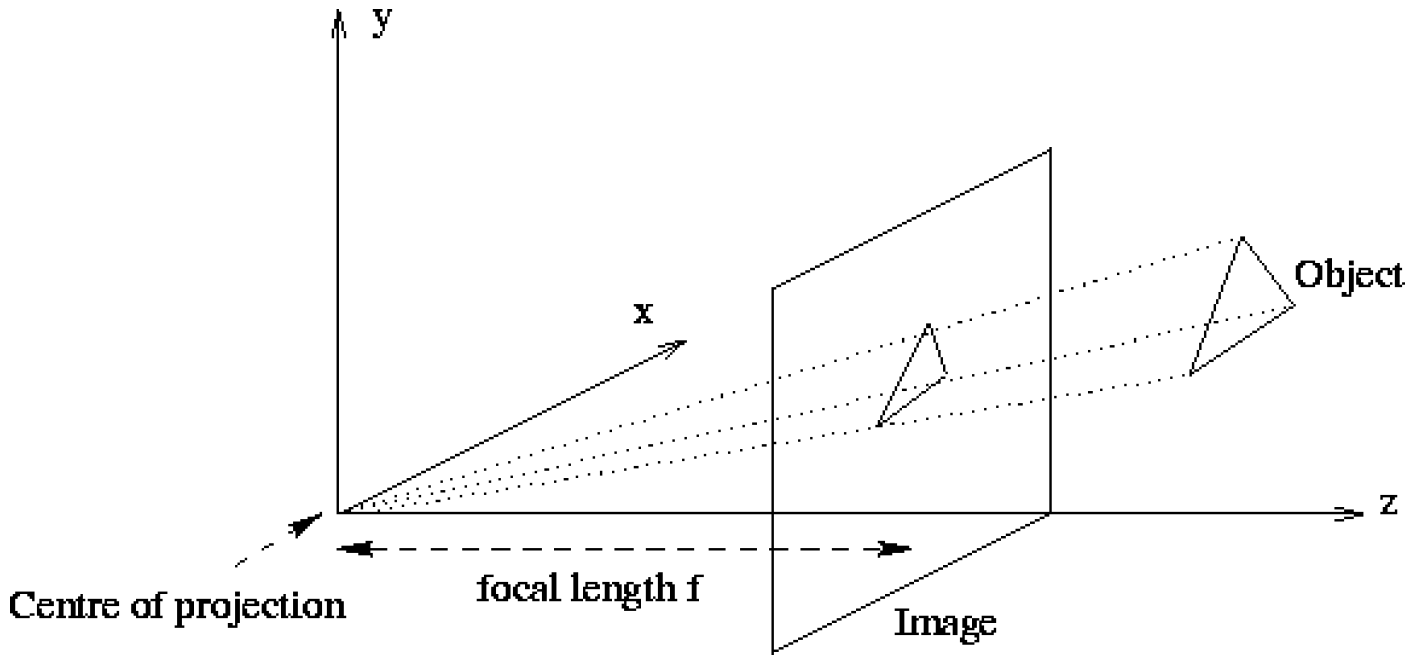
\includegraphics[width=1\linewidth]{Images/lochkameramodell_positivlage.PNG}
\end{myfigure}

The perspective transformation $\pi$ from camera coordinates $\boldsymbol{X}$ to image coordinates $x$ is given by
\begin{equation*}
    \pi : \mathbb{R}^3 \rightarrow \mathbb{R}^2; \quad \boldsymbol{X} \mapsto x = \pi (\boldsymbol{X}) = \begin{pmatrix}f \frac{X}{Z}\\ f \frac{Y}{Z} \end{pmatrix}.
\end{equation*}
In homogeneous coordinates
\begin{equation*}
	Z\boldsymbol{x} = Z\begin{psmallmatrix} x\\ y\\ 1 \end{psmallmatrix} = K_f \Pi_0 \boldsymbol{X}
					= \begin{psmallmatrix} f & 0 & 0 & 0\\0 & f & 0 & 0\\0 & 0 & 1 & 0\end{psmallmatrix} \begin{psmallmatrix} X\\ Y\\ Z\\ 1 \end{psmallmatrix}		
\end{equation*}
with ($\Pi_0$: standard projection matrix)
\begin{equation*}
	K_f = \begin{psmallmatrix} f & 0 & 0\\0 & f & 0\\0 & 0 & 1\end{psmallmatrix} \text{  and  } \Pi_0 = \begin{psmallmatrix} 1 & 0 & 0 & 0\\0 & 1 & 0 & 0\\0 & 0 & 1 & 0\end{psmallmatrix}.
\end{equation*}
Assume $Z = \lambda = \text{const.} > 0$, then
\begin{equation*}
	\lambda \boldsymbol{x} = K_f \Pi_0 \boldsymbol{X}.
\end{equation*}

\textbf{Transform. from world to image coordinates:}\\
Transformation of point $\boldsymbol{X}_0$ in world coordinates to a point $\boldsymbol{X}$ in camera coordinates:
\begin{equation*}
	\boldsymbol{X} = g \boldsymbol{X}_0 = \begin{psmallmatrix} R & T\\0 & 1\end{psmallmatrix} \boldsymbol{X}_0.
\end{equation*}
Transformation from world coordinates to image coordinates:
\begin{equation*}
	\lambda \boldsymbol{x} = K_f \Pi_0 g \boldsymbol{X}_0.
\end{equation*}
By normalizing the focal length $f$ to $1$ (by changing image coordinate units), you get
\begin{equation*}
	\lambda \boldsymbol{x} = \Pi_0 \boldsymbol{X} = \Pi_0 g \boldsymbol{X}_0.
\end{equation*}

\subsection{Intrinsic Camera Parameters} \label{subsection:intrinsic_parameters}
The pixel coordinates $(x', y', 1)$ as a function of homogeneous camera coordinates $\boldsymbol{X}$ are given by
\begin{equation*}
	\lambda \boldsymbol{x}' = \lambda \begin{pmatrix} x'\\y'\\1 \end{pmatrix} = K_s K_f \Pi_0 \boldsymbol{X} = K \Pi_0 \boldsymbol{X}
\end{equation*}
with ($K$: intrinsic parameter matrix)
\begin{equation*}
	K_s = \begin{pmatrix} s_x & s_{\theta} & o_x\\0 & s_y & o_y\\0 & 0 & 1\end{pmatrix} \text{  and  } K = \begin{pmatrix}fs_x & fs_{\theta} & o_x\\0 & fs_y & o_y\\0 & 0 & 1 \end{pmatrix}
\end{equation*}
and as function of world coordinates $\boldsymbol{X}_0$ by
\begin{equation*}
	\lambda \boldsymbol{x}' = K \Pi_0 \boldsymbol{X} = K \Pi_0 g \boldsymbol{X}_0 \equiv \Pi \boldsymbol{X}_0.
\end{equation*}
The matrix $\Pi \equiv K \Pi_0 g = (KR,KT)$ is the general projection matrix.\par
\vspace{4mm}

\textbf{Summary:} (for homogeneous coordinates)\\
4D world coordinates $\boldsymbol{X}_0$ $\xrightarrow{g \, \in \, SE(3)}$ 4D camera coordinates $\boldsymbol{X}$ $\xrightarrow{K_f \Pi_0}$ 3D image coordinates $\boldsymbol{x}$ $\xrightarrow{K_s}$ 3D pixel coordinates $\boldsymbol{x'}$.\par
\vspace{4mm}

The origin for image coordinates is in the center of the 2D image plane with expansion $(-1, -1)$ and $(1, 1)$.\\
The origin of pixel coordinates is moved to the bottom- or top-left corner to enable a purely positive expansion e.g. $(0, 0)$ and $(1024, 768)$.\par
\vspace{4mm}
	
The entries of the intrinsic camera parameter matrix $K$ can be interpreted as follows:
\begin{itemize}
    \item $f$: focal length
    \item $s_x$: scaling to pixels in x-direction
    \item $s_y$: scaling to pixels in y-direction
    \item $s_{\theta}$: skew factor if pixels are not perfectly rectangular (often neglected through $0$)
    \item $fs_x = \alpha_x$: size of unit length in horizontal pixels
    \item $fs_y = \alpha_y$: size of unit length in vertical pixels
    \item $\alpha_x / \alpha_x$: aspect ration $\sigma$
    \item $fs_{\theta}$: skew of the pixel, often close zo zero
    \item $o_x$: x-coordinate of principal point (image center) in pixels
    \item $o_y$: y-coordinate of principal point (image center) in pixels
\end{itemize}
Whereas the extrinsic parameters refer to the camera motion $g = \begin{pmatrix}R & T\\0 & 1 \end{pmatrix}$.

\subsection{Spherical Projection}
Instead of a planar projection surface, one can consider a spherical projection surface given by the unit sphere $\mathbb{S}^2 = \{x \in \mathbb{R}^3 \ \vert \ |x|=1\}$.
The spherical projection $\pi_s$ of a 3D point $\boldsymbol{X}$ is given by:
\begin{equation*}
    \pi_s: \mathbb{R}^3 \rightarrow \mathbb{S}^2; \quad \boldsymbol{X} \mapsto \boldsymbol{x} = \frac{\boldsymbol{X}}{|\boldsymbol{X}|}
\end{equation*}
The whole projection equation
\begin{equation*}
    \lambda \boldsymbol{x}' = K \Pi_0 g \boldsymbol{X}_0
\end{equation*}
is similar to the previous one except for $\lambda = |\boldsymbol{X}| = \sqrt{X^2 + Y^2 + Z^2}$.

\subsection{Radial Distortion}
A simple effective model for distortions along the radial axis is:
\begin{flalign*}
    x &= x_d(1 + a_1r^2 + a_2r^4) \\
    y &= y_d(1 + a_1r^2 + a_2r^4) \\
    r &= x_d^2 + y_d^2
\end{flalign*}
where $\boldsymbol{x}_d \equiv (x_d, y_d)$ is the distorted point, $r$ the radius and $a_1$ and $a_2$ are parameters estimated during calibration. \\
A more general model with an arbitrary center of distortion $c$ is
\begin{equation*}
    \boldsymbol{x} = c + f(r)(\boldsymbol{x}_d - c) \quad \text{with} \quad r = |\boldsymbol{x}_d - c| 
\end{equation*}
\begin{equation*}
    \text{and} \quad f(r) = 1 + a_1r+a_2r^2+a_3r^3 + a_4 r^4.
\end{equation*}

\subsection{Preimage and Coimage}
Due to the unknown scale factor, each point is mapped not to a single point $\boldsymbol{x}$, but to an equivalence class of points $\boldsymbol{y} \sim \boldsymbol{x}$.
\begin{myfigure}
	\centering
	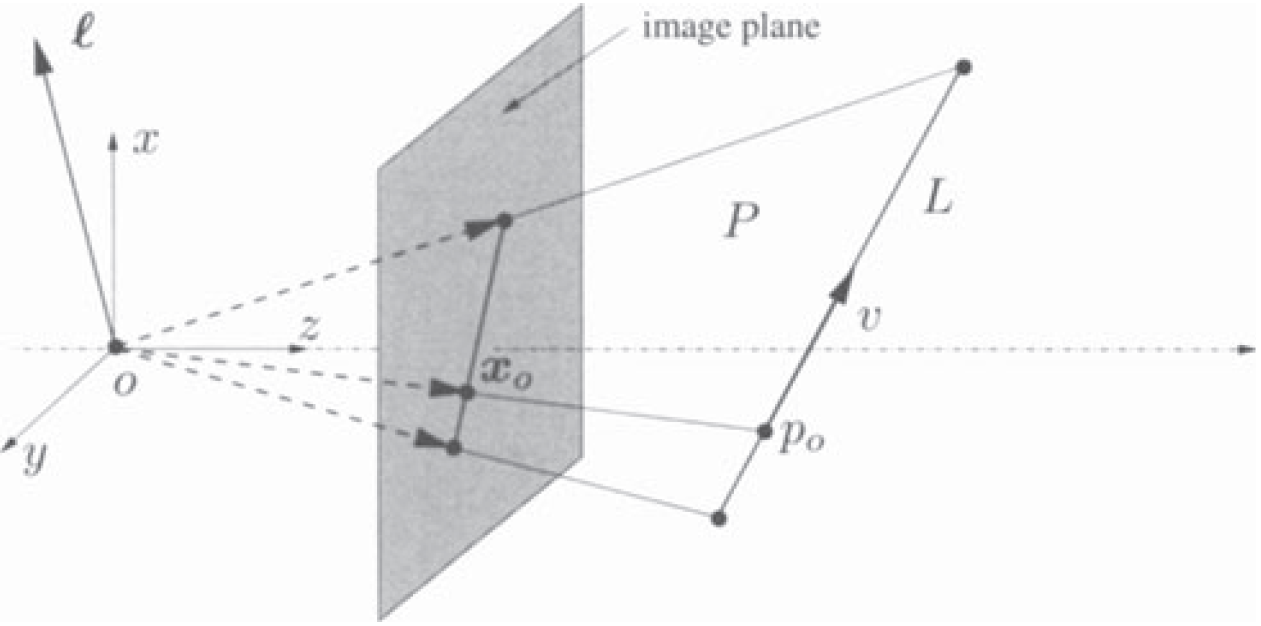
\includegraphics[width=0.8\linewidth]{Images/preimage.PNG}
\end{myfigure}
A line $L$ in 3D is characterized by a base point $\boldsymbol{X}_0 = (X_0, Y_0, Z_0, 1)^T \in \mathbb{R}^4$ and a vector $\boldsymbol{V} = (V_1, V_2, V_3, 0)^T \in \mathbb{R}^4$:
\begin{equation*}
    \boldsymbol{X} = \boldsymbol{X}_0 + \mu \boldsymbol{V} \subset \mathbb{R}^4, \quad \mu \in \mathbb{R}
\end{equation*}
The image of the line $L$ is given by
\begin{equation*}
    \boldsymbol{x} \sim \Pi_0 \boldsymbol{X} = \Pi_0(\boldsymbol{X}_0 + \mu \boldsymbol{V}) = \Pi_0 \boldsymbol{X}_0 + \mu \Pi_0 \boldsymbol{V}
\end{equation*}
All points $\boldsymbol{x}$ treated as vectors from the origin $o$ span a 2D subspace $P$.
The intersection of this plane $P$ with the image plane gives the image of the line.
$P$ is called the preimage of the line.\\
A preimage of a point or a line in the image plane is the largest
set of 3D points that give rise to an image equal to the given
point or line.\par
\vspace{11pt}
The coimage of a point or a line is the subspace in $\mathbb{R}^3$ that is the unique orthogonal complement, i.e. the normal vector, of its preimage.
Image, preimage and coimage are equivalent.\par

In the case of a line $L$ with its 2D preimage, we have
\begin{equation*}
    \boldsymbol{\ell}^T \boldsymbol{x} = 0 \text{  and  } P = \text{span}(\hat{\boldsymbol{\ell}}).
\end{equation*}
$\boldsymbol{\ell} \in \mathbb{R}^3$ is the normal vector to the preimage (2D subspace) of line $L$ and $\text{span}(\hat{\boldsymbol{\ell}})$ is the span of row vectors of $\hat{\boldsymbol{\ell}}$.

\vspace{1mm}
\renewcommand{\arraystretch}{1.3}%
\begin{tabularx}{\linewidth}{|c|Y|Y|Y|}
    \hline
     & Image & Preimage & Coimage \\ \hline
     Point & $\text{span}(\boldsymbol{x}) \, \cap \text{im. plane}$ & $\text{span}(\boldsymbol{x}) \subset \mathbb{R}^3$ & $\text{span}(\hat{\boldsymbol{x}}) \subset \mathbb{R}^3$ \\ \hline
     Line & $\text{span}(\hat{\boldsymbol{\ell}}) \, \cap \text{im. plane}$ & $\text{span}(\hat{\boldsymbol{\ell}}) \subset \mathbb{R}^3$ & $\text{span}(\boldsymbol{\ell}) \subset \mathbb{R}^3$ \\ \hline
\end{tabularx}
\renewcommand{\arraystretch}{1.0}%

\subsection{Projective Geometry}
One can represent 3D points by a general 4D vector $X = (XW, YW, ZW, W) \in \mathbb{R}^4$ remembering that only the direction of this vector is of importance.
We therefore identify the point in homogeneous coordinates with the line connecting it with the origin.
\end{multicols}
\newpage

\begin{multicols}{2}[\section{Estimating Point Correspondence}]
\subsection{From Photometry to Geometry}
In practice, instead of points or lines we observe characteristic image features like brightness or color values at individual pixels. By selecting a small number of feature points from each image, we throw away a large amount of potentially useful information.\\
Two cases are distinguished in point matching: small deformation and wide baseline stereo (large displacement).

\subsection{Small Deformation \& Optical Flow}
The optic flow refers to the apparent 2D motion field observable between consecutive images of a video.
It is different from the motion of objects in the scene. 

\subsubsection{The Lucas-Kanade method}
The Lucas-Kanade method generates sparse flow vectors under the assumption of constant motion in a local neighborhood.\par
\vspace{5pt}
\textbf{Assumptions:}
\begin{itemize}
	\item Let $x(t)$ denote a moving point at time $t$, and $I(x,t)$ a video sequence.
	\item Brightness Constancy assumption (Optical flow constraint): The brightness of point $x(t)$ is constant. $I(x(t),t) = \text{const.}, \, \forall t$ and $\frac{d}{dt}I(x(t),t) = \nabla I^T \cdot \frac{dx}{dt} + \frac{\partial I}{\partial t} = 0$.
	\item Constant motion in a neighborhood: $v$ is constant over a neighborhood $W(x)$ of the point $x$. $\nabla I(x',t)^T v + \frac{\partial I}{\partial t}(x',t) = 0, \, \forall x' \in W(x)$.
\end{itemize}

The least square error of point $x$ is
\begin{flalign*}
    E(v) &= \int_{W(x)} | \nabla I(x',t)^T v + I_t (x',t)|^2 dx' \\
    &= v^T M v + 2 q^T v.
\end{flalign*}
The desired local flow vector (velocity) can be calculated by setting $\frac{dE}{dv} = 0$ and is given by
\begin{equation*}
	v = \frac{dx}{dt} = -M^{-1}q
\end{equation*}
if $M$ is invertible (i.e. $\det(M) \neq 0$) with
\begin{flalign*}
    M &= \int_{W(x)} \nabla I \nabla I^T \;\mathrm{d}x', \quad q = \int_{W(x)} I_t \nabla I \;\mathrm{d}x' \\
    \nabla I &= \begin{pmatrix}I_x \\I_y \end{pmatrix} = \begin{pmatrix}\frac{\partial I}{\partial x} \\ \frac{\partial I}{\partial y} \end{pmatrix}, \quad I_t = \frac{\mathrm{d}I}{\mathrm{d}t}.
\end{flalign*}
$M$ is positive semi-definite.\\

Explicit expressions for $v \in \mathbb{R}^2$:
\begin{equation*}
    v = \begin{pmatrix} \frac{m_{22} q_1 - m_{12} q_2}{m_{12}^2 - m_{11} m_{22}} \\ \frac{m_{11} q_2 - m_{12} q_1}{m_{12}^2 - m_{11} m_{22}} \end{pmatrix}
\end{equation*}
\textbf{Aperture problem:}\\
It is impossible to determine the motion $v$ orthogonal to the gradient direction $\nabla I$ in regions with constant gradient direction.

\subsubsection{Simple feature tracking algorithm (KLT-Tracker)}
\begin{enumerate}
    \item For a given time instance $t$, compute at each point $x \in \Omega$ the structure tensor
    \begin{equation*}
    M(x) = \int_{W(x)} \begin{pmatrix}I_x^2 & I_xI_y\\I_xI_y & I_y^2 \end{pmatrix} \;\mathrm{d}x'.
    \end{equation*}
    \item Mark all points $x \in \Omega$ for which the determinant of $M$ is larger than a threshold $\theta > 0$:
    \begin{equation*}
         \det(M(x)) \geq \theta
    \end{equation*}
    \item For all these points the local velocity is given by:
    \begin{equation*}
        b(x, t) = -M(x)^{-1} \begin{pmatrix}\int I_xI_t \;\mathrm{d}x'\\ \int I_yI_t \;\mathrm{d}x' \end{pmatrix}.
    \end{equation*}
    \item Repeat the above steps for the points $x+b$ at time $t+1$.
\end{enumerate}

\subsubsection{Robust Feature Point Extraction (Harris corner detector)}
One classical feature detector is based on the structure tensor 
\begin{flalign*}
    M(x) &\equiv G_{\sigma} * \nabla I \nabla I^T \\
    &= \int G_{\sigma}(x-x') \begin{pmatrix}I_x^2 & I_xI_y\\I_xI_y & I_y^2 \end{pmatrix}(x') \;\mathrm{d}x' \\
    \text{and } q &= G_{\sigma} * I_t \nabla I
\end{flalign*}
where rather than simple summing over the window $W(x)$ we perform a summation weighted by a Gaussian $G$ of width $\sigma$.
Additionally, the scoring function
\begin{equation*}
    C(x) = \det(M) - \kappa \ \text{Tr}^2(M)
\end{equation*}
and select points for which $C(x) > \theta$ with a threshold $\theta > 0$.

\subsection{Wide Baseline Matching}
In the case of wide baseline matching, large parts of the image plane will not match at all because they are not visible in the other image.\\
Required extensions in comparison to the KLT-Tracker:
\begin{itemize}
	\item Generalize the motion model from translational motions to for example affine motions.
	\item To be more robust to illumination changes replace the sum-of-squared-differences by the normalized cross correlation.
\end{itemize}
Normalized Cross Correlation:
\begin{myfigure}
	\centering
	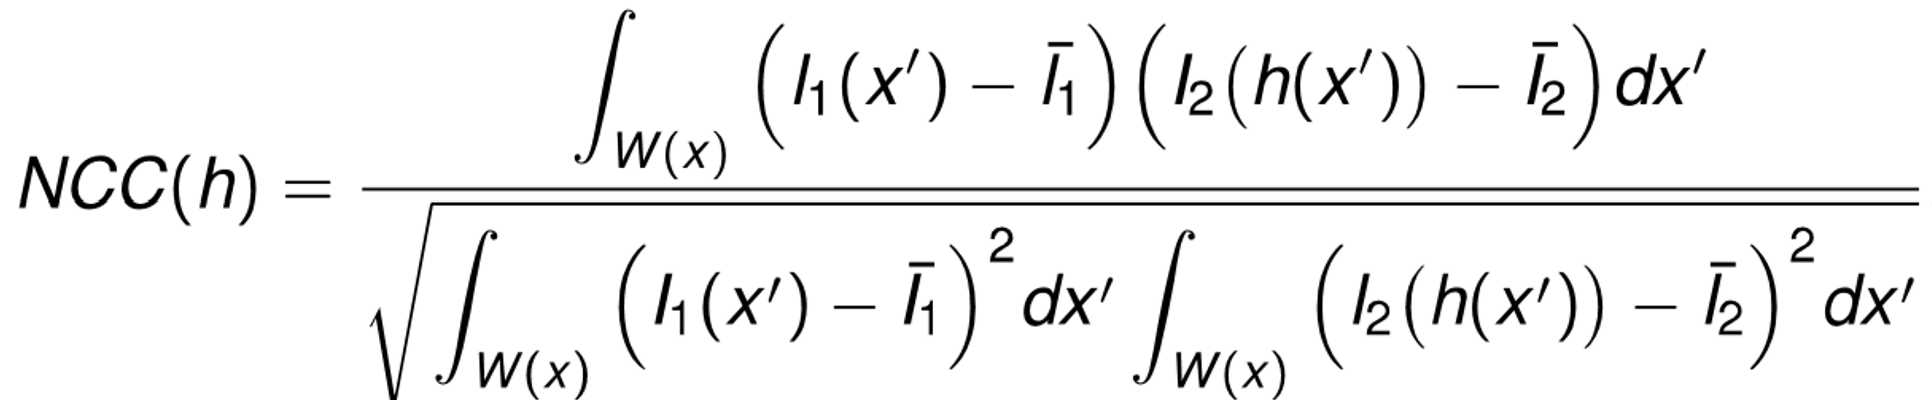
\includegraphics[width=1\linewidth]{Images/ncc.png}
\end{myfigure}
$\bar{I_1}$ and $\bar{I_2}$ are the avg. intensity over $W(x)$.\\
By subtracting this avg. intensity, the measure becomes invariant to additive intensity changes $I \rightarrow I + \gamma$.
By dividing by the intensity variances of each window, the measure becomes invariant to multiplicative intensity changes $I \rightarrow \gamma I$.\par
Often the affine transformation $h(x) = Ax + d$ is used with $\hat{A}, \hat{d} = \underset{A,d}{\mathrm{argmax}} \, NCC(A,d)$.
\end{multicols}

\begin{multicols}{2}[\section{Reconstruction from Two Views: Linear Algorithms}]
\subsection{The Reconstruction Problem}
Assumptions:
\begin{itemize}
	\item A set of corresponding points in two frames from the same camera is given.
	\item The scene is static.
	\item Intrinsic camera parameters are known.
\end{itemize}
3D reconstruction can be done by minimizing the bundle adjustment (re-)projection error:
\begin{flalign*}
	E(R,&T,X_1,...,X_N) = \\
	&= \sum_{j=1}^N || x_1^j - \pi(X_j)||^2 + || x_2^j - \pi(R,T,X_j)||^2
\end{flalign*}
Notation:
\begin{myfigure}
 \centering
 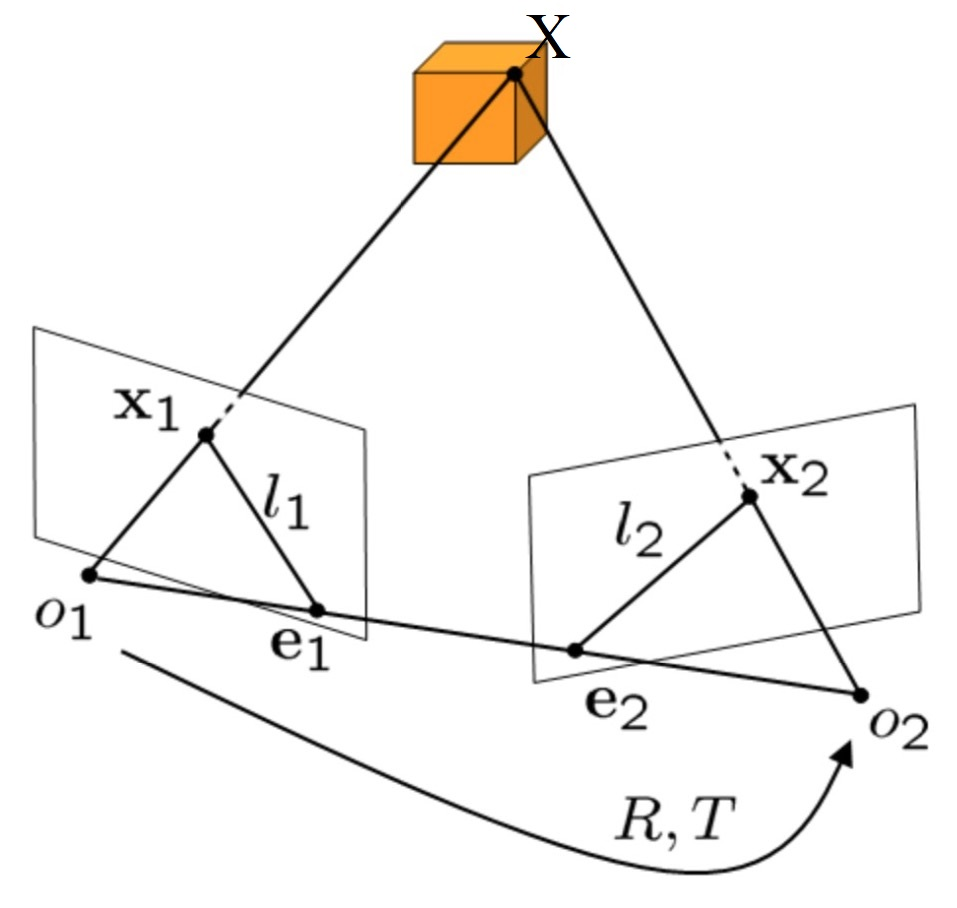
\includegraphics[width=0.65\linewidth]{Images/Epipolar_geometry.jpg}
\end{myfigure}
\begin{itemize}
    \item $X$: point in coordinate system of camera 1
    \item $x_1$ and $x_2$: projections of a point $X$ onto the two images
    \item $o_1$ and $o_2$: optical centers of each camera
    \item $e_1$ and $e_2$: epipoles are the intersections of the line $(o_1, o_2)$ with each image plane
    \item $l_1$ and $l_2$: epipolar lines are the intersections between the epipolar plane $(o_1,o_2,X)$ and the image planes
    \item $\overrightarrow{o_1x}$, $\overrightarrow{o_1o_2}$, $\overrightarrow{o_2x}$ form the epipolar plane. For the volume (triple product) of the corresponding parallelepiped follows $x_2^T(T \times R x_1) = x_2^T \hat{T} R x_1 = 0$.
    \item Further properties: $F e_1 = 0$, $e_2^T F = 0$ (with the fundamental matrix $F$, see Subsection \ref{ssec:the_uncalibrated_case}).
    \item Coimage of epipolar lines: $l_1 \sim E^T x_2$, $l_2 \sim E x_2$
\end{itemize}

\subsection{The Epipolar Constraint}
Assuming known camera parameters ($K=1$) and no rotation or translation of the first camera, we get
\begin{equation*}
    \lambda_1 x_1 = X \quad \text{and} \quad \lambda_2 x_2 = RX+T
\end{equation*}
with unknown depths $\lambda_1$ and $\lambda_2$.
From that one can derive the epipolar constraint
\begin{equation*}
    x_2^T \hat{T} R x_1 = 0.
\end{equation*}
Geometrically, this constraint states that $\overrightarrow{o_1x}$, $\overrightarrow{o_1o_2}$, $\overrightarrow{o_2x}$ form a plane.
The matrix
\begin{equation*}
    E = \hat{T}R \in \mathbb{R}^{3 \times 3}
\end{equation*}
is called the essential matrix.
The space of all essential matrices is called the essential space $\mathcal{E} = \{\hat{T} R \; \vert \; R \in SO(3), T \in \mathbb{R}^3\}$. \par
\vspace{3mm}

\textbf{Essential matrix:}\\
A nonzero matrix $E \in \mathbb{R}^{3 \times 3}$ is an essential matrix if and only if $E$ has a SVD $E = U \Sigma V^T$ with $\Sigma = \text{diag}\{\sigma, \sigma, 0\}$ for some $\sigma > 0$ and $U, V \in SO(3)$.\par

For $E = U \Sigma V^T$ we have:
\begin{equation*}
\begin{split}
    (\hat{T_1}, R_1) = \left(U R_Z (+\frac{\pi}{2})\Sigma U^T, \ U R_Z^T (+\frac{\pi}{2})V^T \right)\\
    (\hat{T_2}, R_2) = \left(U R_Z (-\frac{\pi}{2})\Sigma U^T, \ U R_Z^T (-\frac{\pi}{2})V^T \right)
\end{split}
\end{equation*}
In general, only one of these gives meaningful (positive) depth values.

\subsection{Eight-Point Algorithm}
Procedure:
\begin{enumerate}
    \item Recover the essential matrix $E$ from the epipolar constraints associated with a set of point pairs.
    \item Extract the relative translation and rotation from the essential matrix $E$.
\end{enumerate}
Let
\begin{equation*}
		E^s = (e_{11}, e_{21}, e_{31}, e_{12}, e_{22}, e_{32}, e_{13}, e_{23}, e_{33})^T \in \mathbb{R}^9   
\end{equation*}
be the stack of $E$ and
\begin{equation*}
\begin{split}
    a \equiv \boldsymbol{x}_1 \otimes \boldsymbol{x}_2 = (x_1x_2, x_1y_2, x_1z_2, \\ y_1x_2, y_1y_2, y_1z_2, z_1x_2, z_1y_2, z_1z_2)^T \in \mathbb{R}^9
\end{split}
\end{equation*}
the Kronecker product of the vectors $\boldsymbol{x}_i =(x_i,y_i,z_i)$. \\
Then the epipolar constraint can be written as:
\begin{equation*}
    x_2^T E x_1 = a^T E^s = 0
\end{equation*}
For $n$ point pairs, we can combine this into the linear system ($\chi \in \mathbb{R}^{n \times 9}$):
\begin{equation*}
    \chi E^s = 0, \ \text{with } \chi = (a^1, a^2, \dots, a^n)^T
\end{equation*}
To get a unique solution, we need $\text{rank}(\chi) = 8$ and therefore at least 8 point pairs.
In certain degenerated cases, the solution is not unique even if we have 8 or more point pairs (e.g. when all points lie on a line or on a plane).\\\par

\textbf{Projecting onto essential space:}
The numerically estimated coefficients $E^s$ will in general not correspond to an essential matrix. One can resolve this problem by projecting it back to the essential space $\mathcal{E}$.\\
Let $F \in \mathbb{R}^{3 \times 3}$ be an arbitrary matrix with SVD $F = U \, \text{diag}\{\lambda_1, \lambda_2, \lambda_3\} \, V^T, \ \lambda_1 \geq \lambda_2 \geq \lambda_3$.
Then the essential matrix $E$ minimizing the Frobenius norm $\left\| F - E \right\|_f^2$ is given by
\begin{equation*}
    E = U \cdot \text{diag}\{\sigma, \sigma, 0\} \cdot V^T, \ \text{with } \sigma = \frac{\lambda_1 + \lambda_2}{2} 
\end{equation*}
\paragraph{Complete Eight Point Algorithm (Longuet-Higgins 1981)} \mbox{}\\
Given a set of $n = 8$ or more point pairs $x_1^i$, $x_2^i$:
\begin{enumerate}
    \item \textit{Compute an approximation of the essential matrix.}\\
    Construct the matrix $\chi = (a^1, a^2, \dots, a^n)^T$, where $a^i = x_1^i \otimes x_2^i$. Find the vector $E^s \in \mathbb{R}^9$ which minimizes $||\chi E^s||$ as the ninth column of $V_{\chi}$ in the SVD $\chi = U_{\chi} \Sigma_{\chi} V_{\chi}^T $. Unstack $E^s$ into $3 \times 3$-matrix $E$.
    \item \textit{Project onto essential space.}\\
    Compute the SVD $E = U \, \text{diag}\{\sigma_1, \sigma_2, \sigma_3\} \, V^T$. Since in the reconstruction, $E$ is only defined up to a scalar, we project $E$ onto the normalized essential space by replacing the singular values $\sigma_1$, $\sigma_2$, $\sigma_3$ with $1$, $1$, $0$.
    \item \textit{Recover the displacement from the essential matrix.}\\
    The four possible solutions for rotation and translation are:
    \begin{equation*}
    \begin{split}
        R = U R_Z^T \, (\pm \frac{\pi}{2}) V^T, \\ \hat{T} = U R_Z(\pm \frac{\pi}{2})\Sigma U^T
    \end{split}
    \end{equation*}
    with a rotation by $\pm \frac{\pi}{2}$ around $z$:
    \begin{equation*}
        R_Z \, (\pm \frac{\pi}{2}) = \begin{pmatrix} 0 & \mp 1 & 0\\ \pm 1 & 0 & 0\\0 & 0 & 1 \end{pmatrix}
    \end{equation*}
\end{enumerate}
\subsection{Structure Reconstruction}
In the linear eight-point algorithm, the essential matrix $E$ and hence the translation $T$ are only defined up to an arbitrary scale $\gamma \in \mathbb{R}^{+}$, with $\left\| E \right\| = \left\| T \right\| = 1$. Combining all unknown scale parameters $\vec{\lambda} = \left(\lambda_1^1, \lambda_1^2, \dots , \lambda_1^n, \gamma\right)^T \in \mathbb{R}^{n+1}$, we get the linear equation system
\begin{equation*}
	\begin{split}
		M \vec{\lambda} = 0 \text{\quad with \qquad \qquad} \\
		M \equiv
		\begin{psmallmatrix}
			\widehat{\boldsymbol{x}}_2^1 R \boldsymbol{x}_1^1 & 0 & 0 & 0 & 0 & \widehat{\boldsymbol{x}}_2^1 T \\
			0 & \widehat{\boldsymbol{x}}_2^2 R \boldsymbol{x}_1^2 & 0 & 0 & 0 & \widehat{\boldsymbol{x}}_2^2 T \\
			0 & 0 & \ddots & 0 & 0 & \vdots \\
			0 & 0 & 0 & \widehat{\boldsymbol{x}}_2^{n-1} R \boldsymbol{x}_1^{n-1} & 0 & \widehat{\boldsymbol{x}}_2^{n-1} T \\
			0 & 0 & 0 & 0 & \widehat{\boldsymbol{x}}_2^n R \boldsymbol{x}_1^n & \widehat{\boldsymbol{x}}_2^n T
		\end{psmallmatrix}
	\end{split}
\end{equation*}
The linear least squares estimate for $\vec{\lambda}$ (only defined up to an arbitrary scale) is given by the eigenvector corresponding to the smallest eigenvalue of $M^TM$. \\

The eight-point algorithm only provides unique solutions (up to a scalar factor) if all 3D points are in a ''general position''.
This is no longer the case for certain degenerate configurations, for which all points lie on certain 2D surface such as walls or floors.

\subsection{Four Point Algorithm}
If $\boldsymbol{X}_1 \in \mathbb{R}^3$ denotes point coordinates in the first frame, and these lie on a plane with normal $N \in \mathbb{S}^2$ ($N^T \boldsymbol{X}_1 = d$), then we have:
\begin{flalign*}
    \boldsymbol{X}_2 &= H \boldsymbol{X}_1 \text{ with } H = R + \frac{1}{d}TN^T \in \mathbb{R}^{3 \times 3} \\
    \lambda_2 \boldsymbol{x}_2 &= H \lambda_1 \boldsymbol{x}_1 \text{ (in 2D homog. image coordinates)}
\end{flalign*}
where $H$ is called a homography matrix.
By multiplying with $\widehat{\boldsymbol{x}_2}$, we get to the planar epipolar (or homography) constraint:
\begin{equation*}
    \widehat{\boldsymbol{x}_2} H \boldsymbol{x}_1 = 0
\end{equation*}
Again, we can cast this equation into the form $\boldsymbol{a}^TH^s = 0$ with $H^s = (H_{11}, H_{21}, \dots, H_{33})^T \in \mathbb{R}^9$ and $\boldsymbol{a} \equiv \boldsymbol{x}_1 \otimes \widehat{\boldsymbol{x}}_2 \in \mathbb{R}^{9 \times 3}$. \\
Let us now assume we have $n \geq 4$ pairs of corresponding 2D points $\{\boldsymbol{x}_1^j, \boldsymbol{x}_2^j\}, j = 1,\dots , n$, in the two images.
Each point pair induces a matrix $\boldsymbol{a}^j$, we integrate these into a larger matrix $\chi \equiv (\boldsymbol{a}^1, \dots , \boldsymbol{a}^n)^T \in \mathbb{R}^{3n \times 9}$ and obtain the system
\begin{equation*}
    \chi H^s = 0
\end{equation*}

\paragraph{Four Point Algorithm}
\begin{enumerate}
    \item For the point pairs, compute the matrix $\chi$.
    \item Compute a solution $H^s$ for the above equation by SVD of $\chi$.
    \item Extract the motion parameters from the homography matrix $H = R + \frac{1}{d} TN^T$.
\end{enumerate}
From $H$, the parameters $R$, $N$ and $T/d$ can be derived.
The 3D structure of the points can be computed as before.
Relations between essential matrix $E=\hat{T} R$ and homography matrix $H = R + Tu^T$ with some $u \in \mathbb{R}^3$:
\begin{equation*}
    E=\hat{T} H, \quad H^T E + E^T H = 0
\end{equation*}

\subsection{The Uncalibrated Case} \label{ssec:the_uncalibrated_case}
The reconstruction algorithms introduced above all assume that the camera is calibrated ($K = 1$). If the parameters of $K$ are known then one can simply transform the pixel coordinates $\boldsymbol{x}'$ to normalized coordinates $\boldsymbol{x} = K^{-1} \boldsymbol{x}'$ (for $K$ see subsection \ref{subsection:intrinsic_parameters}) to obtain the representation used in the previous sections.\\
Reconstruction from uncalibrated views works with 
\begin{equation*}
    \boldsymbol{x}_2^{' \, T} \, F \, \boldsymbol{x}'_1 = 0
\end{equation*}
with the fundamental matrix defined as
\begin{equation*}
    F \equiv K_2^{-T} \hat{T} R K_1^{-1} = K_2^{-T} E K_1^{-1}
\end{equation*}
$F$ has an SVD $F = U \Sigma V^T$ with $\Sigma = \text{diag}(\sigma_1, \sigma_2, 0)$.
It is not straight forward how to proceed from here.
\end{multicols}

\begin{multicols}{2}[\section{Reconstruction from Multiple Views (skipped)}]
\subsection{From Two Views to Multiple Views}
In this section, we deal with the problem of 3D reconstruction given multiple views of a static scene, either obtained simultaneously, or sequentially from a moving camera.
\subsection{Preimage \& Coimage from Multiple Views}
The preimage of multiple images of points and lines can be defined by the intersection:
\begin{equation*}
\begin{split}
    preimage(x_1, \dots, x_m)\\ = preimage(x_1) \cap \dots \cap preimage(x_m)\\
    preimage(\ell_1, \dots, \ell_m)\\ = preimage(\ell_1) \cap \dots \cap preimage(\ell_m)
\end{split}
\end{equation*}
\begin{myfigure}
 \centering
 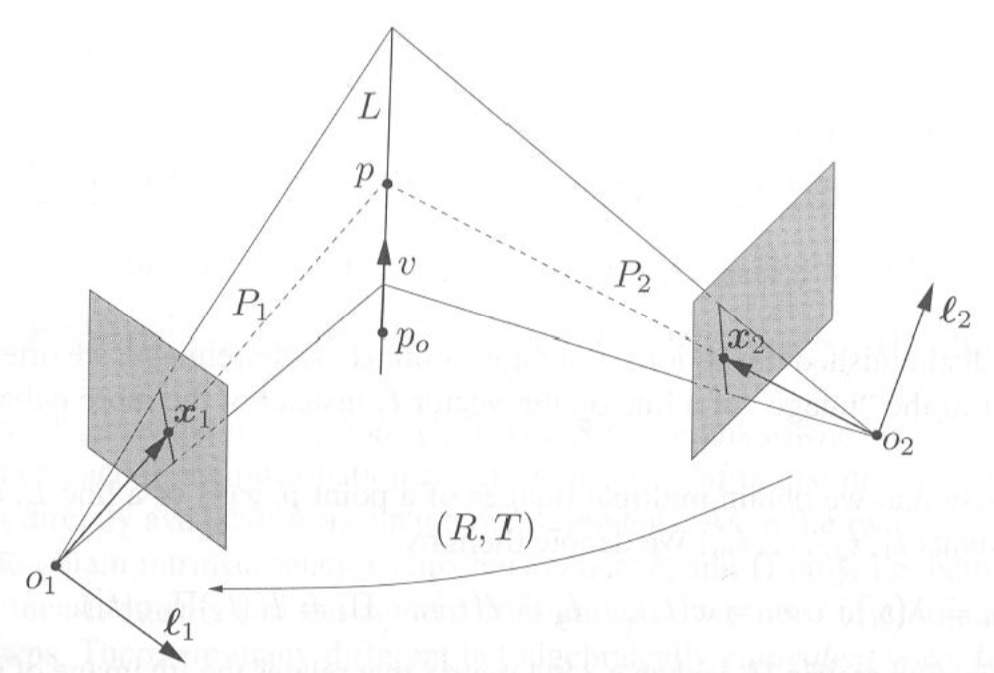
\includegraphics[width=0.8\linewidth]{Images/Preimage.jpg}
 \captionof{figure}{Images of a point $p$ on a line $L$}
\end{myfigure}
\begin{itemize}
    \item Preimages $P1$ and $P2$ of the image lines should intersect in the line $L$; in other words the intersection of the two planes $P1$ and $P2$ is exactly the $3D$ line $L$
    \item Preimages of the two image points $x_1$ and $x_2$ should intersect in the point $p$.
    \item Normals $l_1$ and $l_2$ to the planes $P1$ and $P2$ define the coimages of the line $L$.
\end{itemize}
\subsection{From Preimages to Rank Constraints}

\paragraph{Point Features} \mbox{}\\
The multiple-view projection matrix $\Pi \in \mathbb{R}^{3m \times 4}$ associated with the image matrix $\mathcal{I} \in \mathbb{R}^{3m \times m}$ gives
\begin{equation*}
\begin{split}
    N_p \equiv (\Pi, \mathcal{I}) = \begin{pmatrix} \Pi_1 & x_1 & 0 & \dots & 0\\ \Pi_2 & 0 & x_2 & 0 &  0\\ \vdots & \vdots & \vdots & \ddots & \vdots\\ \Pi_m & 0 & 0 & \dots & x_m\\\end{pmatrix} \\ \in \mathbb{R}^{3m \times (m+4)}
\end{split}
\end{equation*}
with its implied rank constraint
\begin{equation*}
    \text{rank}(N_p) \leq m + 3
\end{equation*}
Some conversions also lead to
\begin{equation*}
\begin{split}
    W_p \equiv \mathcal{I}^{\perp} \Pi = \begin{pmatrix} \hat{x_1} \Pi_1 \\ \hat{x_2} \Pi_2 \\ \vdots \\ \hat{x_m} \Pi_m \\\end{pmatrix} \in \mathbb{R}^{3m \times 4}
\end{split}
\end{equation*}
plus 
\begin{equation*}
    \text{rank}(W_p) = \text{rank}(N_p) - m \leq 3
\end{equation*}
\paragraph{Line Features} \mbox{}\\
Similarly, 
\begin{equation*}
\begin{split}
    W_l \equiv \begin{pmatrix} \ell_1^T \Pi_1 \\ \ell_2^T \Pi_2 \\ \vdots \\ \ell_m^T \Pi_m \\\end{pmatrix} \in \mathbb{R}^{m \times 4}
\end{split}
\end{equation*}
with the rank constraint
\begin{equation*}
    \text{rank}(W_l) \leq 2
\end{equation*}


\subsection{Geometric Interpretation}
Since all matrices $\hat{x}_i$ have rank 2, the number of independent rows in $W_p$ is at most $2m$. These rows define a set of $2m$ planes. Since $W_p X = 0$, the point $X$ is in the intersection of all these planes.
\begin{myfigure}
 \centering
 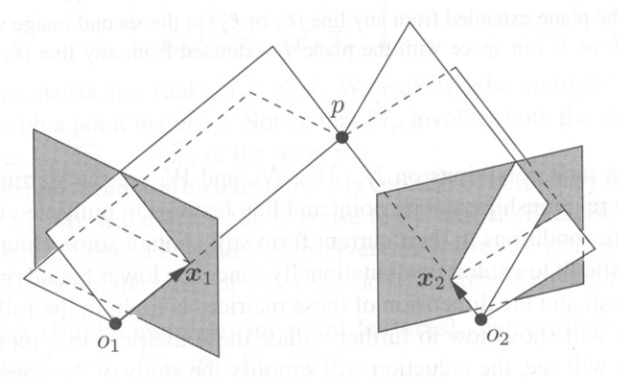
\includegraphics[width=0.9\linewidth]{Images/Preimage_two_image_points.jpg}
 \captionof{figure}{Preimage of two image points}
\end{myfigure}
We already habe $\text{rank}(W_l) \leq 2$, so there is no intrinsic constraint on two images of a line: The preimage of two image lines always contains a line.
\begin{myfigure}
 \centering
 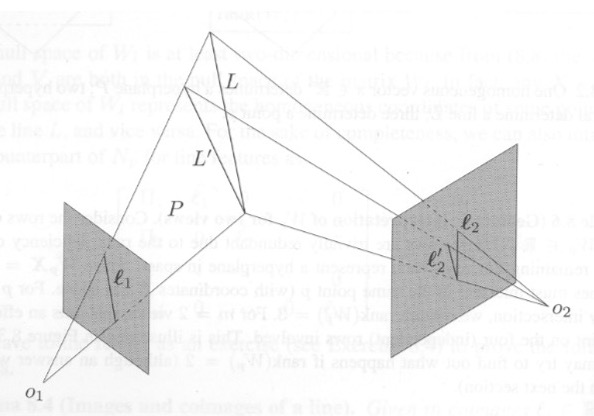
\includegraphics[width=0.9\linewidth]{Images/Preimage_two_image_lines.jpg}
 \captionof{figure}{Preimage of two image lines}
\end{myfigure}

\subsection{The Multiple-view Matrix}
The matrix 
\begin{equation*}
\begin{split}
    M_p \equiv \begin{pmatrix}\hat{x_2}R_2x_1 & \hat{x_2}T_2\\ \hat{x_3}R_3x_1 & \hat{x_3}T_3\\ \vdots & \vdots\\ \hat{x_m}R_mx_1 & \hat{x_m}T_m\\ \end{pmatrix} \\ \in \mathbb{R}^{3(m-1) \times 2}
\end{split}
\end{equation*}
with $\text{rank}(M_p) \leq 1$ is called the multiple-view matrix associated with a point $p$.\\
In summary: For multiple images of a point $p$ the matrices $N_p$, $W_p$ and $M_p$ satisfy:
\begin{equation*}
\begin{split}
    \text{rank}(M_p) = \text{rank}(W_p) -2 = \\ \text{rank}(N_p) - (m +2) \leq 1
\end{split}
\end{equation*}

\subsection{Relation to Epipolar Constraints}
$M_p$ contains geometric information which is the epipolar constraint by \begin{equation*}
    x_i^T \, \hat{T_i} R_i x_1 = 0
\end{equation*}

Furthermore, the trilinear constraint: 
\begin{equation*}
    \hat{x_i} (T_i x_1^T \, R_j^T - R_ix_1T_j^T)\hat{x_j} = 0
\end{equation*}
Let $x_1, x_2, x_3 \in \mathbb{R}^3$ be the 2D point coordinates in three camera frames with distinct optical centers. If the trilinear constraints
\begin{equation*}
\begin{split}
    \hat{x_j} \left(T_{ji} x_i^T R_{ki}^T - R_{ji} x_i T_{ki}^T \right) \hat{x_k} = 0, \\ i, j, k = 1, 2, 3
\end{split}
\end{equation*}
(combination of the two trilinear constraints from above) hold then a unique preimage is determined unless the three lines associated to image points $x1$, $x2$, $x3$ are colinear. 

\begin{myfigure}
 \centering
 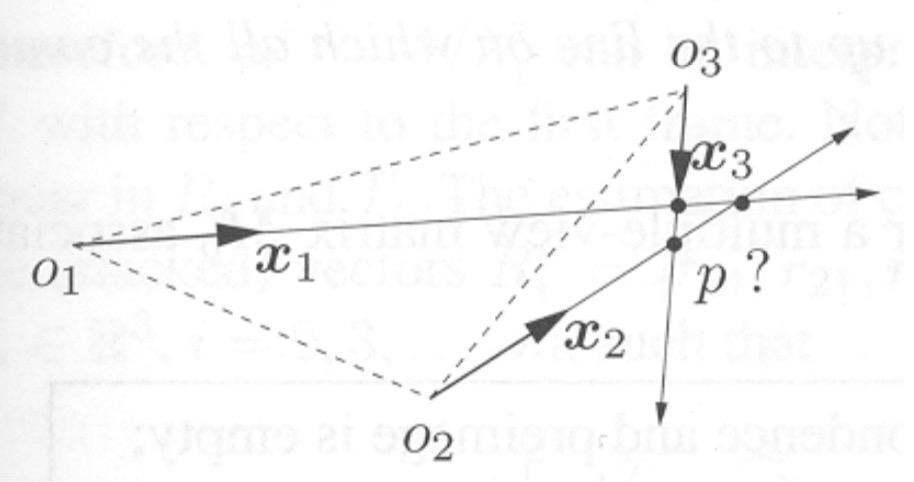
\includegraphics[width=0.9\linewidth]{Images/Degeneracy_trifocal_plane.jpg}
 \captionof{figure}{All pairs of lines intersect, yet it does not imply a unique 3D point $p$ (a unique preimage)}
\end{myfigure}

\begin{myfigure}
 \centering
 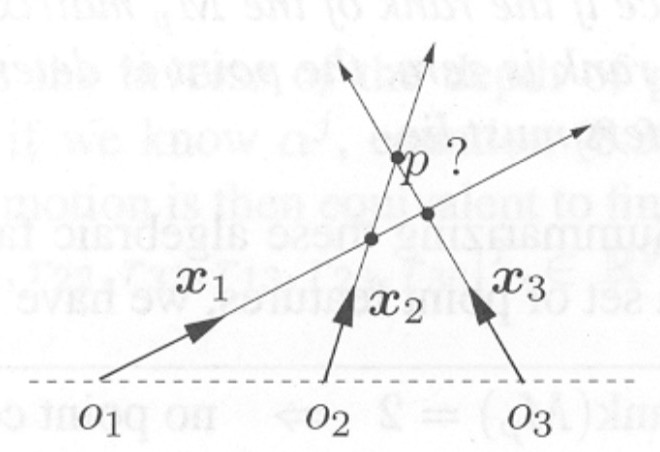
\includegraphics[width=0.9\linewidth]{Images/Degeneracy_rectlinear_motion.jpg}
 \captionof{figure}{Again, all pairs of lines may intersect without there being a unique preimage $p$ - fortunately, the trilinear constraint assures a unique preimage (unless p is also on the same line with the optical centers)}
\end{myfigure}

In summary we get:
\begin{equation*}
\begin{split}
    \text{rank}(M_p) = 2 \Rightarrow \text{no point correspondence} \\ \text{\& empty preimage} \\
    \text{rank}(M_p) = 1 \Rightarrow \text{point correspondence} \\ \text{\& unique preimage} \\
    \text{rank}(M_p) = 0 \Rightarrow \text{point correspondence} \\ \text{\& preimage not unique}
\end{split}
\end{equation*}

\subsection{Multiple-View Factorization of Point Features}
Suppose we have $m$ images $x^j_1 , ... , x^j_m $ of $n$ points $p^i$ and we want to estimate the unknown matrix $\Pi$. To separate the structure and motion an alternating algorithm is performed. 
\\
\\
\textbf{Motion Estimation from Known Structure:} \\
Assume we have the depth of the points and thus their inverse $\alpha^j  = 1/\lambda^j_1$. Then the above equation is linear in the camera motion parameters $R_i$ and $T_i$. 
\begin{center}
    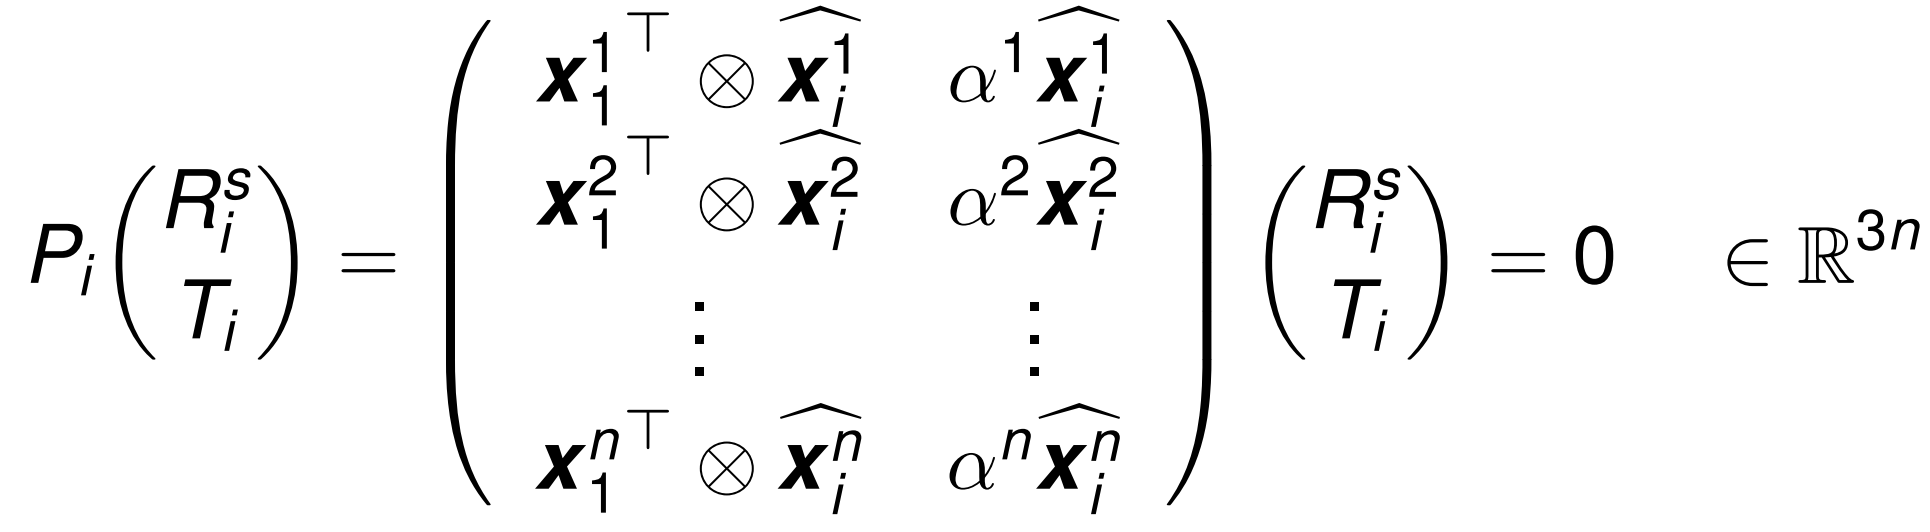
\includegraphics[width=1\linewidth]{Images/Pi.png}
\end{center}
One can show that the matrix $P_i \in \mathbb{R}^{3n \times 12}$ is of rank 11 if more than n=6 points in general position are given. In practice one would use more than 6 points, obtain a full-rank matrix and compute the solution by a singular value decomposition (SVD).
\\
\\
\textbf{Structure Estimation from Known Motion:} \\
If the camera motion is known, one can estimate the structure. The least squares solution for the above equation is given by: 
\begin{center}
    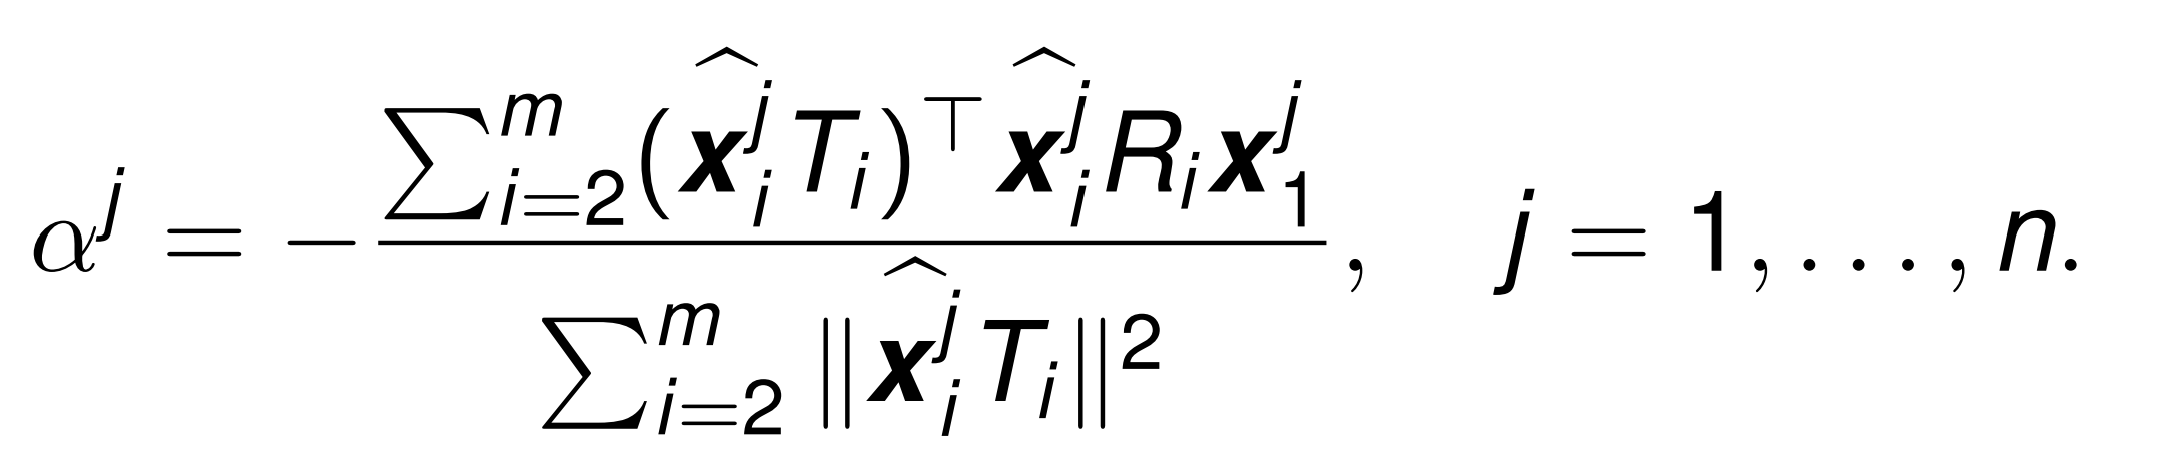
\includegraphics[width=1\linewidth]{Images/alpha.png}
\end{center}
For initialization one could apply the eight-point algorithm to
the first two images to obtain an estimate of the structure
parameters $\alpha^j$.
\subsection{Multiple-View Reconstruction of Lines}
The matrix 
\begin{equation*}
\begin{split}
    M_l \equiv \begin{pmatrix}\ell_2^T \, R_2 \hat{\ell_1} & \ell_2^T \, T_2 \\ \vdots & \vdots \\ \ell_m^T \, R_m \hat{\ell_1} & \ell_m^T \, T_m \\ \end{pmatrix} \\ \in \mathbb{R}^{(m-1) \times 4}
\end{split}
\end{equation*}
has the rank constraint
\begin{equation*}
    \text{rank}(M_l) \leq 1.
\end{equation*}

From the trilinear constraint
\begin{equation*}
    \ell_j^T \, T_j \ell_i^T \, R_i \hat{\ell_1} - \ell_i^T \, T_i \ell_j^T \, R_j \hat{\ell_1} = 0
\end{equation*}
one can conclude that any multiview constraint on lines can be reduced to constraints which only involve three lines at a time.

In general, $\text{rank}(M_l) \leq 1$ if and only if all its 2x2-minors, have zero determinant. Since these minors only include three images at a time, one can conclude that any multiview constraint on lines can be reduced to constraints which only involve three lines at a time.
\paragraph{Lemma} \mbox{}\\
Given three camera frames with distinct optical centers and any three vectors $\ell_1, \ell_2, \ell_3 \in \mathbb{R}^3$ that represent three image lines. If the three image lines satisfy the trilinear constraints
\begin{equation*}
\begin{split}
    \ell_j^T \, T_{ji} \ell_k^T \, R_{ki} \hat{\ell_i} - \ell_k^T \, T_{ki} \ell_j^T \, R_{ji} \hat{\ell_i} = 0, \\ i, j, k \in \{1, 2, 3\}
\end{split}
\end{equation*}
(combination of the two trilinear constraints from above) then their preimage $L$ is uniquely determined except for the case in which the preimage of every $\ell_i$ is the same plane in space. This is the only degenerate case, and in this case, the matrix $M_l$ becomes zero.\\

\begin{myfigure}
 \centering
 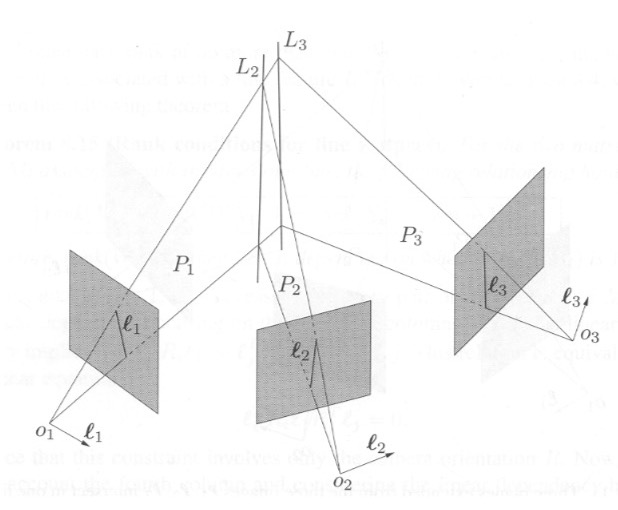
\includegraphics[width=0.8\linewidth]{Images/Preimage_no_line.jpg}
 \captionof{figure}{No preimage: The lines $L_2$ and $L_3$ do not coincide}
\end{myfigure}

\begin{myfigure}
 \centering
 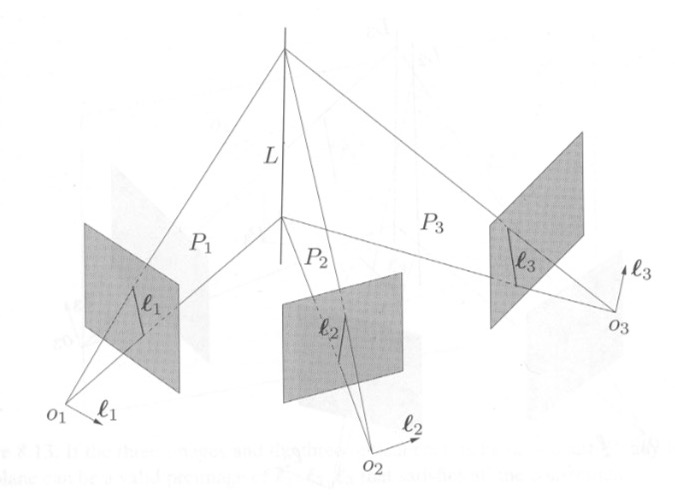
\includegraphics[width=0.8\linewidth]{Images/Preimage_line.jpg}
 \captionof{figure}{Uniqueness of the preimage: The lines $L_2$ and $L_3$ coincide}
\end{myfigure}

Overall we have the following cases:
\begin{equation*}
\begin{split}
    \text{rank}(M_l) = 2 \Rightarrow \text{no line correspondence} \\
    \text{rank}(M_l) = 1 \Rightarrow \text{line correspondence} \\ \text{\& unique preimage} \\
    \text{rank}(M_l) = 0 \Rightarrow \text{line correspondence} \\ \text{\& preimage not unique}
\end{split}
\end{equation*}

\paragraph{Summary} \mbox{}\\
\vspace{1mm} \\
\renewcommand{\arraystretch}{1.1}%
\begin{tabularx}{\linewidth}{|c|Y|Y|Y|}
    \hline
     & (Pre) image &  Coimage & Jointly \\ \hline
     Point & \makecell{$\text{rank}(N_p)$ \\ $\leq m + 3$} & \makecell{$\text{rank}(W_p)$ \\ $\leq 3$}  & \makecell{$\text{rank}(M_p)$ \\ $\leq 1$} \\ \hline
     Line & \makecell{$\text{rank}(N_l)$ \\ $\leq m + 3$} & \makecell{$\text{rank}(W_l)$ \\ $\leq 3$}  & \makecell{$\text{rank}(M_l)$ \\ $\leq 1$} \\ \hline
\end{tabularx}
\renewcommand{\arraystretch}{1.0}%
\vspace{1mm} \\
These rank conditions capture the relationships among corresponding geometric primitives in multiple images. They impose the existence of unique preimages (up to degenerate cases). Moreover, they give rise to natural factorization-based algorithms for multiview recovery of 3D structure and motion (i.e. generalizations of the eight-point algorithm).
\end{multicols}

\begin{multicols}{2}[\section{Bundle Adjustment \& Nonlinear Optimization}]
\subsection{Optimality in Noisy Real World Conditions}
For noisy data $\Tilde{\boldsymbol{x}}_1$, $\Tilde{\boldsymbol{x}}_2$ we have neither a guarantee that $R$ and $T$ are as close as possible to the true solution nor that we will get a consistent reconstruction.

\begin{myfigure}
 \centering
 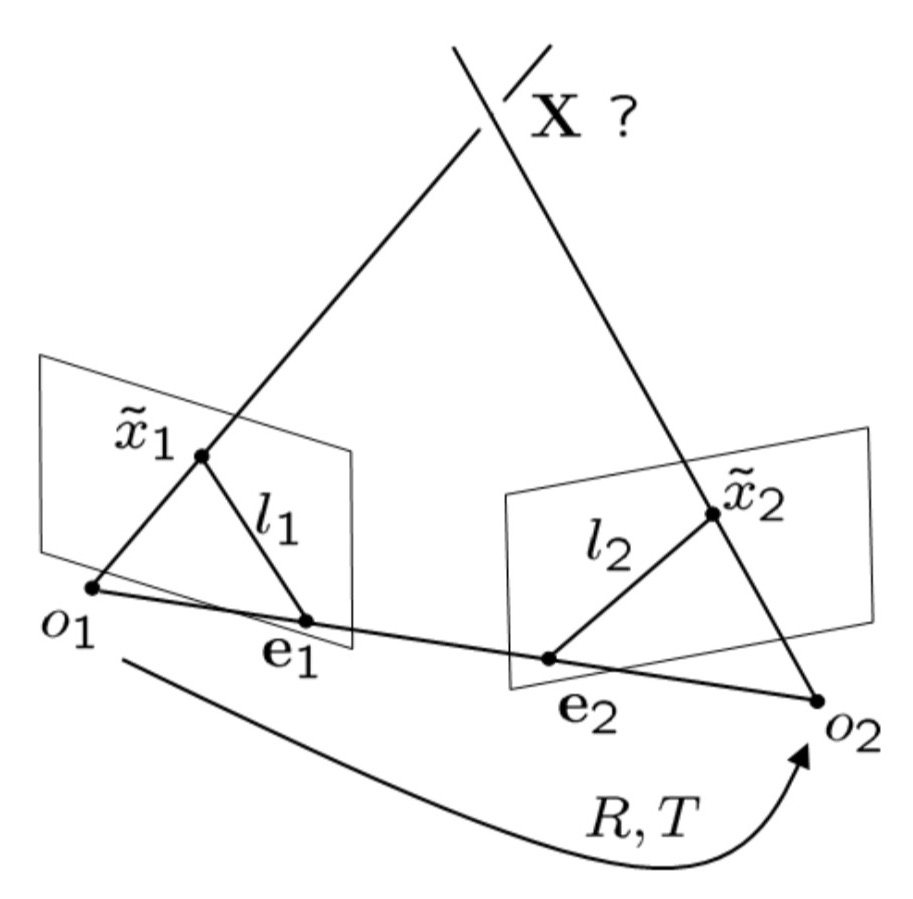
\includegraphics[width=0.7\linewidth]{Images/Camera_motion_noisy.jpg}
\end{myfigure}

Previous linear approaches are elegant because the compute optimal solutions in closed form.
For noisy point locations, they often provide suboptimal performance or even fail.\\
A Bayesian formulation determines the most likely camera transformation $R$, $T$ and 2D coordinates $\boldsymbol{x}$ by performing a maximum aposteriori estimate.
This approach however involves modeling probability densities $\mathcal{P}$ on a fairly complicated space.

\subsection{Bundle Adjustment}
Under the assumption that the observed 2D point coordinates $\Tilde{\boldsymbol{x}}$ are corrupted by zero-mean Gaussian noise, maximum likelihood estimation leads to bundle adjustment:
\begin{equation*}
\begin{split}
    E(R, T, \boldsymbol{X}_1, \ldots, \boldsymbol{X}_N) = \sum_{j = 1}^N | \Tilde{\boldsymbol{x}}_1^j - \pi (\boldsymbol{X}_j)|^2 \\ + | \Tilde{\boldsymbol{x}}_2^j - \pi (R, T, \boldsymbol{X}_j)|^2
\end{split}
\end{equation*}

It aims at minimizing the (re)projection error between the observed 2D coordinates $\Tilde{\boldsymbol{x}}_i^j$ and the projected 3D coordinate $\boldsymbol{X}_j$ with respect to camera 1.

For the general case of $m$ images, we get:
\begin{flalign*}
    E(\{R_i, T_i\}_{i = 1\ldots m}, &\{\boldsymbol{X}_j\}_{j = 1\ldots N}) = \\
    &= \sum_{i = 1}^m \sum_{j = 1}^N \Theta_{i j} |\Tilde{\boldsymbol{x}}_i^j - \pi (R_i, T_i, \boldsymbol{X}_j)|^2
\end{flalign*}
with $T_1 = 0$ and $R_1 = 1$. $\Theta_{ij} = 1$ if point $j$ is visible in image $i$, $\Theta_{ij} = 0$ else. The problems are non-convex. \\ \\

The same optimization problem can be parametrized differently. We introduce $\boldsymbol{x}_i^j$ to denote the true 2D coordinate associated with the measured coordinate $\Tilde{\boldsymbol{x}}_i^j$:
\begin{flalign*}
    E(\{\boldsymbol{x}_1^j, &\lambda_1^j\}_{j = 1 \ldots N}, R, T) = \\
    &= \sum_{j=1}^N ||\boldsymbol{x}_1^j - \Tilde{\boldsymbol{x}}_1^j||^2 + ||\Tilde{\boldsymbol{x}}_2^j - \pi(R \lambda_1^j \boldsymbol{x}_1^j + T)||^2 
\end{flalign*}
Alternatively, a constrained optimization by minimizing the cost function:
\begin{equation*}
    E(\{\boldsymbol{x}_i^j\}_{j=1 \ldots N}, R, T) = \sum_{j=1}^N \sum_{i=1}^2 ||\boldsymbol{x}_i^j - \Tilde{\boldsymbol{x}}_i^j ||^2
\end{equation*}
with constraints for $j = 1, \ldots , N$:
\begin{equation*}
	\begin{split}
		\boldsymbol{x}_2^{j \, T} \hat{T} R \boldsymbol{x}_1^j = 0 \text{ (epipolar constraint)}\\
		\boldsymbol{x}_1^{j \, T} e_3 = 1, \; \boldsymbol{x}_2^{j \, T} e_3 = 1 \text{ (lying on image plane)}
	\end{split}
\end{equation*}

The name "bundle adjustment" is derived from the attempt of adjusting the bundles of light rays emitted from the 3D points. \\
The highly non-convex cost function requires good initialization. Hence, it is used in the last step in a reconstruction pipeline.


\subsection{Nonlinear Optimization}
Nonlinear programming denotes the process of iteratively solving a nonlinear optimization problem, i.e. a problem involving the maximization or minimization of an objective function over a set of real variables under a set of equality or inequality constraints. \\
In the following we will discuss:
\begin{itemize}
    \item Gradient descent,
    \item Newton methods,
    \item Gauss-Newton algorithm,
    \item Levenberg-Marquardt algorithm.
\end{itemize}

\subsection{Gradient Descent}
Gradient descent is a first-order optimization method. It aims at computing a local minimum of a (generally) non-convex cost function by iteratively stepping in the direction in which the energy decreases most. This is given by the negative energy gradient.
\begin{equation*}
    x_{k+1} = x_k - \epsilon \frac{dE}{dx} (x_k) \quad k = 0, 1, 2, \ldots
\end{equation*}
For the case of convex $E$, the found local minimum will also be the global minimum. The step size $\epsilon$ can be chosen differently in each iteration.\\
Gradient descent is very popular, however not the fastest method in most cases.

\begin{myfigure}
 \centering
 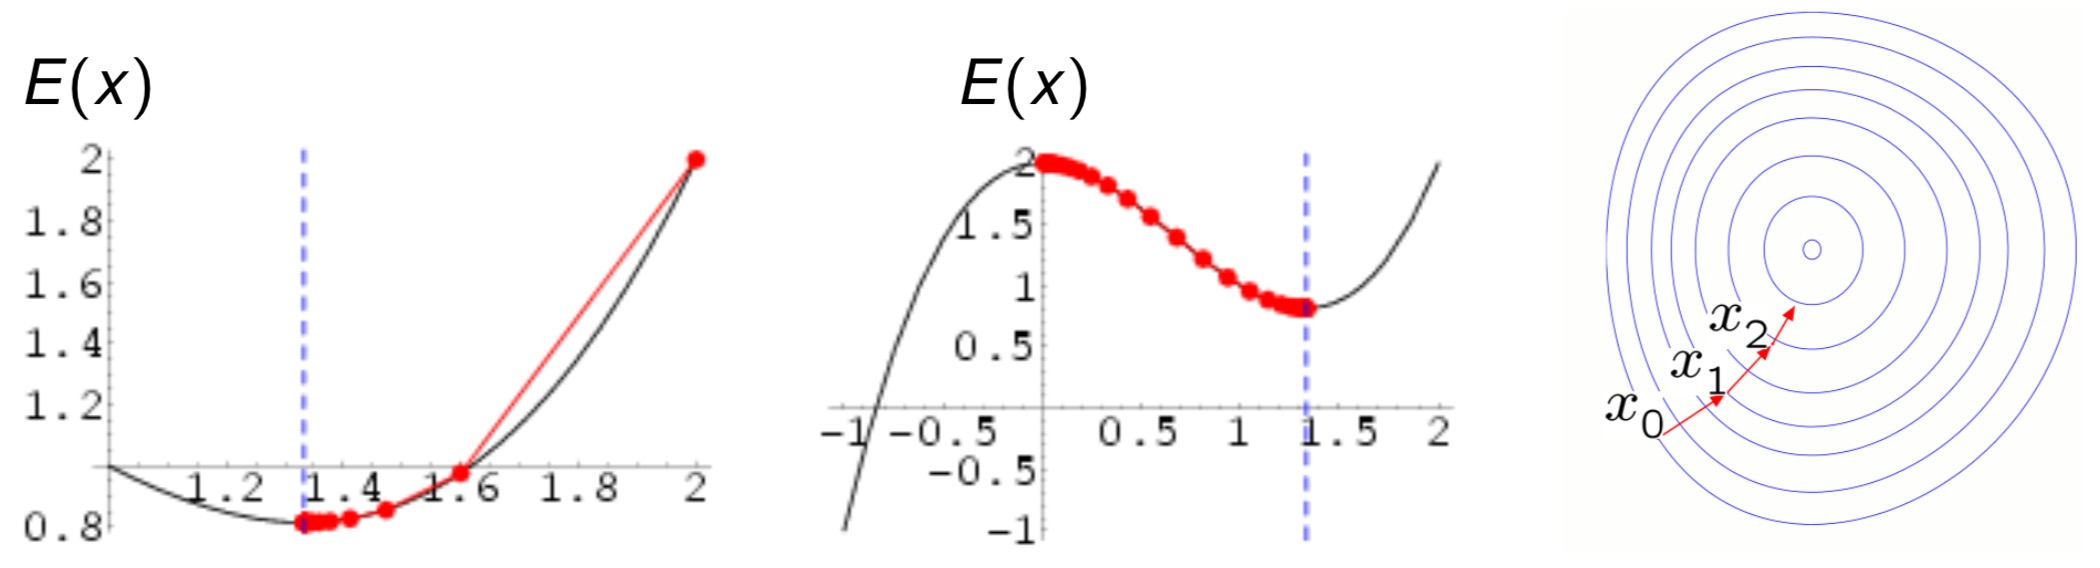
\includegraphics[width=1.0\linewidth]{Images/Gradient_descent.jpg}
\end{myfigure}

\subsection{Least Squares Estimation}
\textbf{Linear (ordinary) least squares} is a method for estimating a set of parameters in a linear regression model.
Assume there is a linear relationship of the form
\begin{equation*}
	a_i = b_i^T x + \eta_i
\end{equation*}
with input $b_i \in \mathbb{R}^d$, output $a_i \in \mathbb{R}$, $i \in \{1,\dots,n\}$, an unknown vector $x \in \mathbb{R}^d$ and zero-mean Gaussian noise $\eta \sim \mathcal{N}(0,\boldsymbol{\Sigma})$, $\boldsymbol{\Sigma} = \sigma^2 \boldsymbol{I_n}$.
The maximum likelihood estimation of $x$ leads to the ordinary least squares problem (convex):
\begin{equation*}
	\min_{x} \sum_{i} (a_i - x^T b_i)^2 = (a-\boldsymbol{B}x)^T (a - \boldsymbol{B}x).
\end{equation*}

For general $\boldsymbol{\Sigma}$, we get the generalized least squares problem:
\begin{equation*}
    \min_{x} (a-\boldsymbol{B}x)^T \boldsymbol{\Sigma}^{-1} (a - \boldsymbol{B}x).
\end{equation*}
This is a quadratic cost function with positive definite $\boldsymbol{\Sigma}^{-1}$.
It has the closed-form solution:
\begin{equation*}
    \hat{x} = (\boldsymbol{B}^T \boldsymbol{\Sigma}^{-1} \boldsymbol{B})^{-1} \boldsymbol{B}^T \boldsymbol{\Sigma}^{-1} a
\end{equation*}

With $\boldsymbol{\Sigma}$ being diagonal (no correlation between variables), we get weighted least squares:
\begin{equation*}
	\min_{x} \sum_{i} w_i (a_i - x^T b_i)^2, \quad \text{with } w_i = \sigma_i^{-2}.
\end{equation*}

For the case of unknown matrix $\boldsymbol{\Sigma}$, there exist iterative estimation algorithms such as feasible generalized least squares or iteratively reweighted least squares.\par

\textbf{Iterative reweighted least squares} aims at minimizing generally non-convex optimization problems of the form
\begin{equation*}
	\min_{x} \sum_i w_i(x) |a_i - f_i(x)|^2,
\end{equation*}
with some known weighting function $w_i(x)$.
A solution is obtained by iterating the following problem:
\begin{equation*}
	x_{t+1} = \text{arg}\min_{x} \sum_i w_i(x_t) |a_i - f_i(x)|^2.
\end{equation*}
For the case that fi is linear, i.e. $f_i(x) = x^T b_i$, each subproblem is simply a weighted least squares problem that can be solved in closed form.
Nevertheless, this iterative approach will generally not converge to a global minimum of the original (nonconvex) problem.\par

\textbf{Nonlinear least squares estimation} aims at fitting observations with a nonlinear model of the form $a_i \approx f(b_i, x)$ for some function $f$ parametrized with an unknown vector $x$.
Minimizing the sum of squares error
\begin{equation*}
    \min_{x} \sum_i r_i (x)^2, \quad \text{with} \quad r_i(x)=a_i-f(b_i,x)
\end{equation*}
is generally a non-convex optimization problem. The optimality condition is given by
\begin{equation*}
    \sum_i r_i \frac{\partial r_i}{\partial x_j} = 0, \quad \forall j \in \{1,...,d\}.
\end{equation*}
Typically one uses iterative algorithms to solve these equation.


\subsection{Newton Methods}
Newton methods are second-order methods that make use of the second derivative.
Let $x_t$ be the estimated solution after $t$ iterations.
Then the Taylor approximation of the cost function $E(x)$ in the vicinity of this estimate is (1. Fitting the parabola):
\begin{equation*}
\begin{split}
    E(x) \approx E(x_t) + g^T (x-x_t) + \frac{1}{2} (x-x_t)^T \boldsymbol{H} (x-x_t)
\end{split}
\end{equation*}
with the Jacobian $g = \frac{dE}{dx}(x_t)$ and the Hessian matrix $\boldsymbol{H} = \frac{d^2E}{dx^2}(x_t)$.
The optimality condition is (2. Going to minimum of parabola in each iteration):
\begin{equation*}
    \frac{dE}{dx} = g + \boldsymbol{H} (x-x_t) = 0
\end{equation*}
Setting the next iterate to the minimizer $x$ leads to:
\begin{equation*}
    x_{t+1} = x_t - \boldsymbol{H}^{-1} g.
\end{equation*}
Requirement: $\boldsymbol{H}$ has to be positive definite.\\
When applicable, second-order methods are often faster than first-order methods, at least when measured in number of iterations.\\
For large optimization problems, computing and inverting the Hessian may be challenging.


\subsection{The Gauss-Newton Algorithm}
The Gauss-Newton algorithm is a method to solve nonlinear least-squares problems of the form:
\begin{equation*}
    \min_{x} \sum_i r_i (x)^2
\end{equation*}
It is an approximation of the Newton method (dropping second order derivative) which with
\begin{equation*}
    H \approx 2\boldsymbol{J}^T \boldsymbol{J} \quad \text{with the Jacobian } \boldsymbol{J} = \frac{dr}{dx} 
\end{equation*}
together with $g = 2\boldsymbol{J}^T r$ leads to the Gauss-Newton algorithm:
\begin{flalign*}
    x_{t+1} &= x_t + \Delta \\ \Delta &= -(\boldsymbol{J}^T \boldsymbol{J})^{-1} \boldsymbol{J}^T r.
\end{flalign*}
In contrast to the Newton algorithm, the Gauss-Newton algorithm does not require the computation of second derivatives.
This approximation of the Hessian is valid if the residuum $r_i$ is small or if it is close to
linear.


\subsection{The Levenberg-Marquardt Algorithm}
The Newton algorithm can be modified (damped)
\begin{equation*}
    x_{t+1} = x_t - (\boldsymbol{H} + \lambda \boldsymbol{I}_n)^{-1} g
\end{equation*}
to create a hybrid between the Newton method ($\lambda = 0$) and a gradient descent with step size $\frac{1}{\lambda}$ (for $\lambda \rightarrow \infty$).\\
In the same manner Levenberg suggested to damp the Gauss-Newton algorithm for nonlinear least squares:
\begin{flalign*}
    x_{t+1} &= x_t + \Delta \\ \Delta &= -(\boldsymbol{J}^T \boldsymbol{J} + \lambda \boldsymbol{I}_n)^{-1} \boldsymbol{J}^T r
\end{flalign*}
Marquardt suggested a more adaptive component-wise damping of the form 
\begin{equation*}
    \Delta = -(\boldsymbol{J}^T \boldsymbol{J} + \lambda \cdot \text{diag}(\boldsymbol{J}^T \boldsymbol{J}))^{-1} \boldsymbol{J}^T r
\end{equation*}
which avoids slow convergence in directions of small gradient.

\subsection{Summary}
Bundle adjustment aims at estimating the locations of $N$ 3D points $X_j$ and camera motions ($R_i$,$T_i$), given noisy 2D projections $\Tilde{x}_i^j$ in $m$ images.\\
The solution to the weighted nonlinear least squares problem (non-convex) can be computed by various iterative algorithms, most importantly the Gauss-Newton algorithm or its damped version, the Levenberg-Marquardt algorithm.\\
Bundle adjustment is typically initialized by an algorithm such as the eight-point or five-point algorithm.
\end{multicols}

\begin{multicols}{2}[\section{Direct Approaches to Visual SLAM}]
In the past chapters we have studied classical approaches to multiple view reconstruction.
These methods tackle the problem of structure and motion estimation (visual SLAM) in several steps:
\begin{enumerate}
    \item A set of feature points is extracted from the images (e.g. corners).
    \item Determine a correspondence of these points across the various images by local tracking (using optical flow approaches) or by random sampling of possible partners based on a feature descriptor (SIFT, SURF, etc.) associated with each point.
    \item The camera motion is estimated based on a set of corresponding points (e.g. eight-point algorithm followed by bundle adjustment).
    \item For a given camera motion one can then compute a dense reconstruction using stereo reconstruction methods.
\end{enumerate}

Such classical approaches are \textbf{indirect} in the sense that they do not compute structure and motion directly from the images but rather from a sparse set of precomputed feature points.\\
\vspace{3mm}

\textbf{Drawbacks:}
\begin{itemize}
	\item Suboptimalilty from the point of view of statistical inference: In the selection of feature points much potentially valuable information contained in the colors of each image is discarded.
	\item Lack of robustness: Errors in the point correspondence may have devastating effects on the estimated camera motion. Since one often selects very few point pairs only (e.g. 8 points for the eight-point algorithm), any incorrect correspondence will lead to an incorrect motion estimate.
	\item Not addressing the highly coupled problems of motion estimation and dense structure estimation. Indirect approaches merely do so for a sparse set of points. As a consequence, improvements in the estimated dense geometry will not be used to improve the camera motion estimates.
\end{itemize}

\subsection{Direct Methods}
Direct methods aim at estimating camera motion and dense or semi-dense scene geometry directly from the input images.\\
\vspace{3mm}

\textbf{Advantages:}
\begin{itemize}
\item More robust to noise and other nuisances because all available input information is exploited.
\item Provide a semi-dense geometric reconstruction of the scene which goes well beyond the sparse point cloud generated by the eight-point algorithm or bundle adjustment. Depending on the application, a separate dense reconstruction step may no longer be necessary.
\item Typically faster because the feature-point extraction and correspondence finding is omitted: Direct approaches can provide fairly accurate camera motion and scene structure in real-time on a CPU.
\end{itemize}
\begin{myfigure}
 \centering
 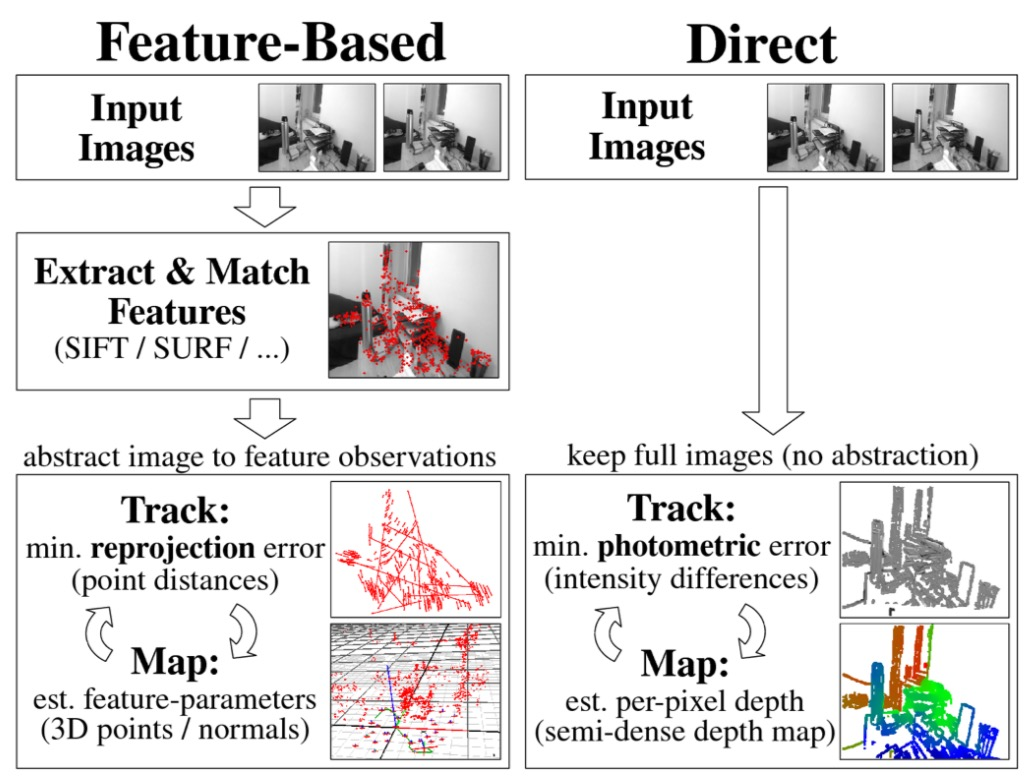
\includegraphics[width=0.9\linewidth]{Images/Comparison_feature_based_direct.jpg}
\end{myfigure}

\subsection{Realtime Dense Geometry}
Let $g_i \in SE(3)$ be the rigid body motion from the first camera to the $i$-th camera, and let $I_i: \Omega \rightarrow \mathbb{R}$ be the $i$-th image.
A dense depth map $h: \Omega \rightarrow \mathbb{R}$ can be computed by solving the optimization problem: 
\begin{equation*}
\begin{split}
    \min_h \sum_{i=2}^n \int_{\Omega} |I_1(x) - I_i(\pi g_i (hx)) | \;\mathrm{d}x \\  + \lambda \int_{\Omega} |\nabla h| \;\mathrm{d}x
\end{split}
\end{equation*}
where a pixel $x \in \Omega$ is represented in homogeneous coordinates and $hx$ is
the corresponding 3D point.\\
The transformation into the other images $I_i$ should give rise to the same color as in the reference image $I_1$. 
\begin{myfigure}
	\centering
	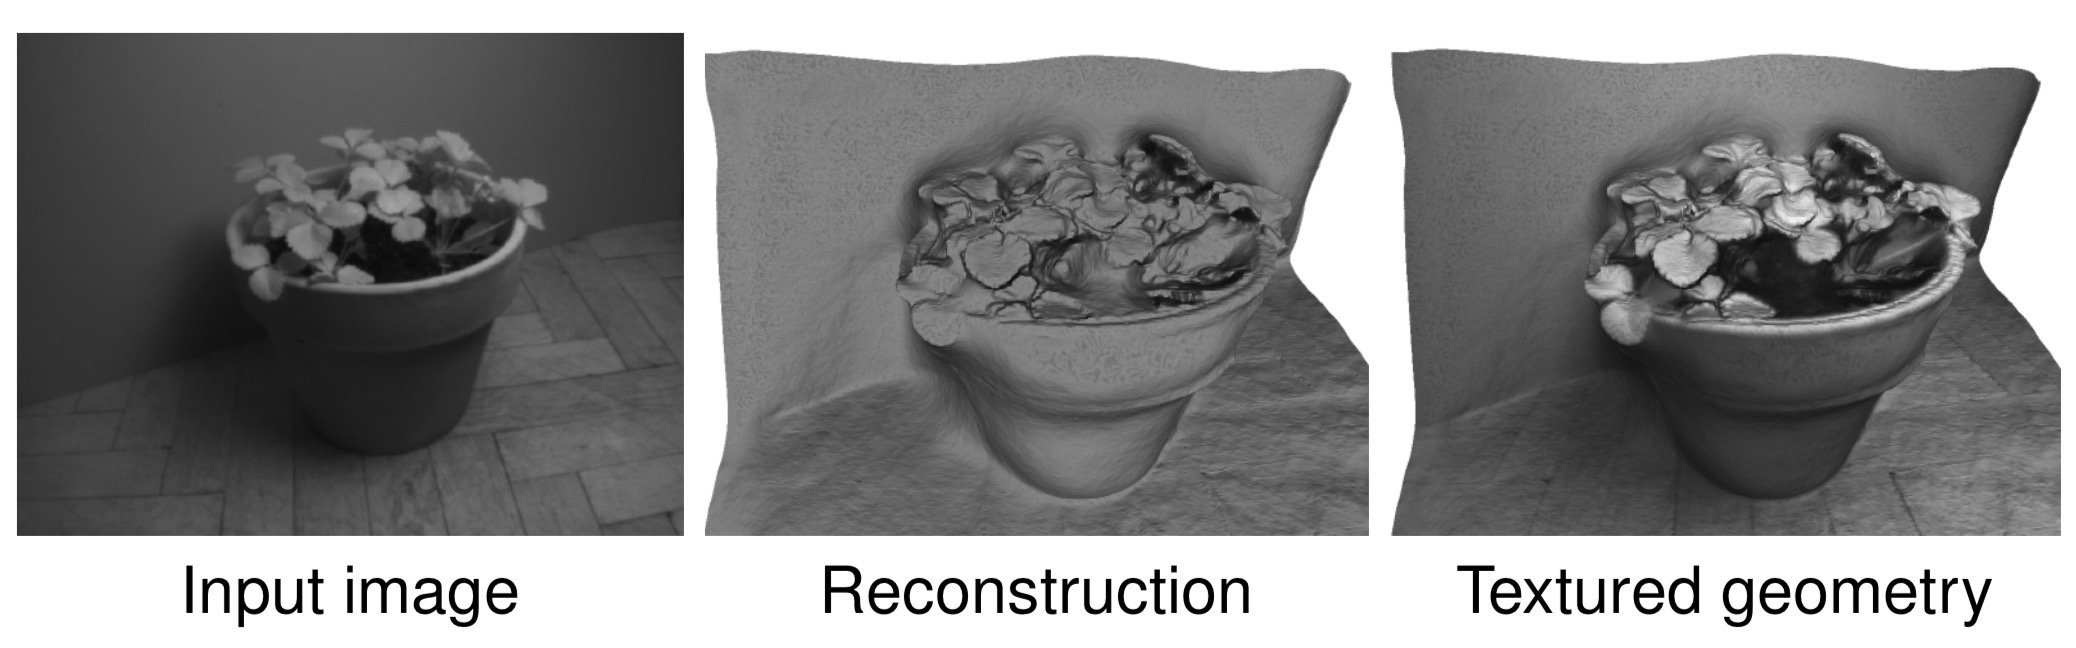
\includegraphics[width=0.9\linewidth]{Images/Realtime_dense_geometry.jpg}
\end{myfigure}
The approach (Stuehmer, Gumhold, Cremers, DAGM 2010) relies on a sparse feature-point based camera tracker (PTAM) to calculate $g_i$ and computes dense geometry directly on the images. 

\subsection{Dense RGB-D Tracking}
Steinbruecker, Sturm, Cremers (2011) propose a complementary approach to directly compute the camera motion from RGB-D images.
The idea is to compute the rigid body motion $g_{\xi}$ which optimally aligns two subsequent color images $I_1$ and $I_2$:
\begin{equation*}
	\min_{\xi \in se(3)} \int_{\Omega} |I_1(x) - I_2(\pi g_{\xi}(hx))|^2 \;\mathrm{d}x
\end{equation*}

\begin{myfigure}
 \centering
 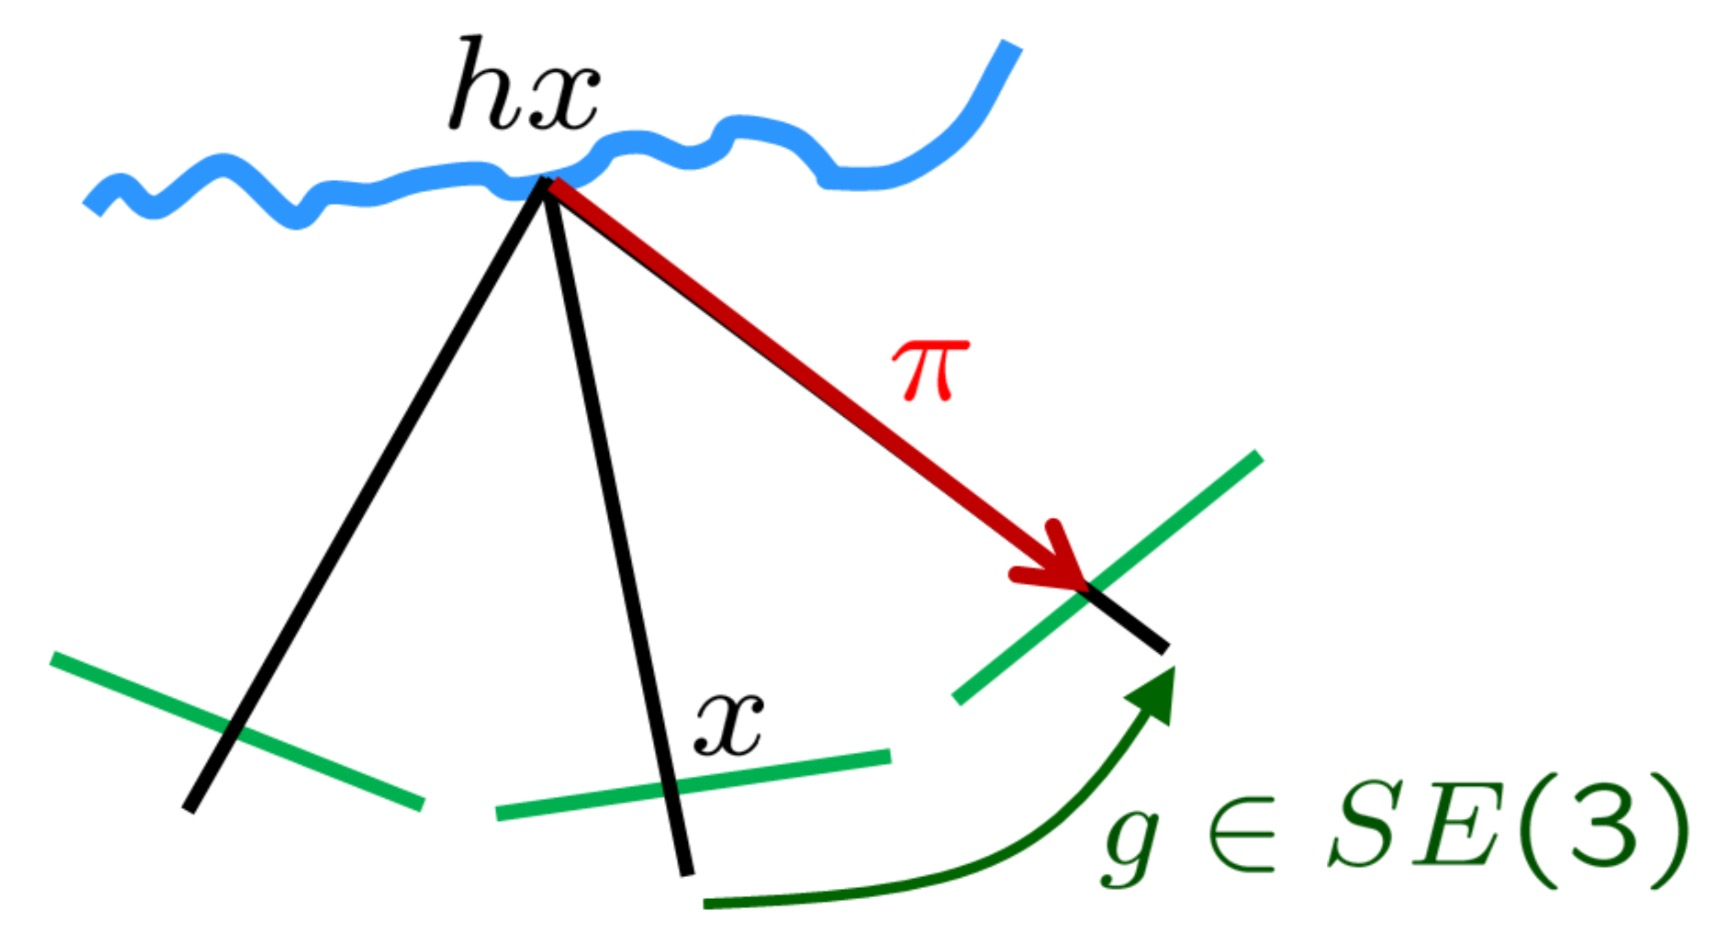
\includegraphics[width=0.9\linewidth]{Images/Dense_RGB-D_Tracking.jpg}
\end{myfigure}
The above non-convex problem can be approximated as a convex problem by linearizing the residuum around an initial guess $\xi_0$:
\begin{equation*}
    \Scale[0.92]{E(\xi) \approx \int_{\Omega} \left| I_1(x) - I_2(\pi g_{\xi_0} (hx)) - \nabla I_2^T \left(\frac{d\pi}{dg_{\xi}} \right) \left(\frac{dg_{\xi}}{d \xi} \right) \xi \right|^2 \mathrm{d}x}
\end{equation*}
This is a convex quadratic cost function which gives rise to a linear optimality condition:
\begin{equation*}
    \frac{d E(\xi)}{d \xi} = A \xi + b = 0
\end{equation*}
For small camera motions, this image aligning approach provides more accurate camera motion than the commonly used generalized Iterated Closest Points (GICP) approach.\\ \\

\subsection{Combining Photometric and Geometric Consistency}
Kerl, Sturm, Cremers, IROS 2013 propose an extension of the RGB-D camera tracker which combines color consistency and geometric consistency of subsequent RGB-D images.
Assuming that the vector $r_i = (r_{ci}, r_{zi}) \in \mathbb{R}^2$ containing the color and geometric (depth) discrepancy for pixel $i$ follows a bivariate t-distribution, the maximum likelihood pose estimate can be computed as (nonlinear weighted least squares problem):

\begin{equation*}
    \min_{\xi \in \mathbb{R}^6} \sum_i w_i r_i^T \Sigma^{-1} r_i
\end{equation*}

with weights $w_i$ based on the student t-distribution:
\begin{equation*}
    w_i = \frac{\nu+1}{\nu+r_i^T \Sigma^{-1} r_i}
\end{equation*}
Solvable by alternating a Gauss-Newton style optimization with a re-estimation of the weights $w_i$ and the matrix $\Sigma$.

\subsection{Loop Closure and Global Consistency}
When tracking a camera over a longer period of time, errors tend to accumulate.
While a single room may still be mapped more or less accurately, mapping a larger environment will lead to increasing distortions.\par

Solution: Introduce pose graph optimization and loop closuring.\\
Key idea: Estimate the relative camera motion $\widehat{\xi}_{ij}$ for any camera pair $i$ and $j$ in a certain neighborhood.\\
Subsequently, one can determine a globally consistent camera trajectory $\xi = \{\xi_i\}_{i=1 \ldots T}$ by solving the nonlinear least squares problem
\begin{equation*}
\begin{split}
    \min_{\xi} \sum_{i \sim j} \left(\widehat{\xi}_{ij} - \xi_i \circ \xi_j^{-1} \right)^T \Sigma_{ij}^{-1} \left(\widehat{\xi}_{ij} - \xi_i \circ \xi_j^{-1} \right)
\end{split}
\end{equation*}
where $\Sigma_{ij}^{-1}$ denotes the uncertainty of measurement $\widehat{\Sigma}_{ij}$.
The problem can be solved e.g. by Levenberg-Marquardt algorithm. 

\begin{myfigure}
 \centering
 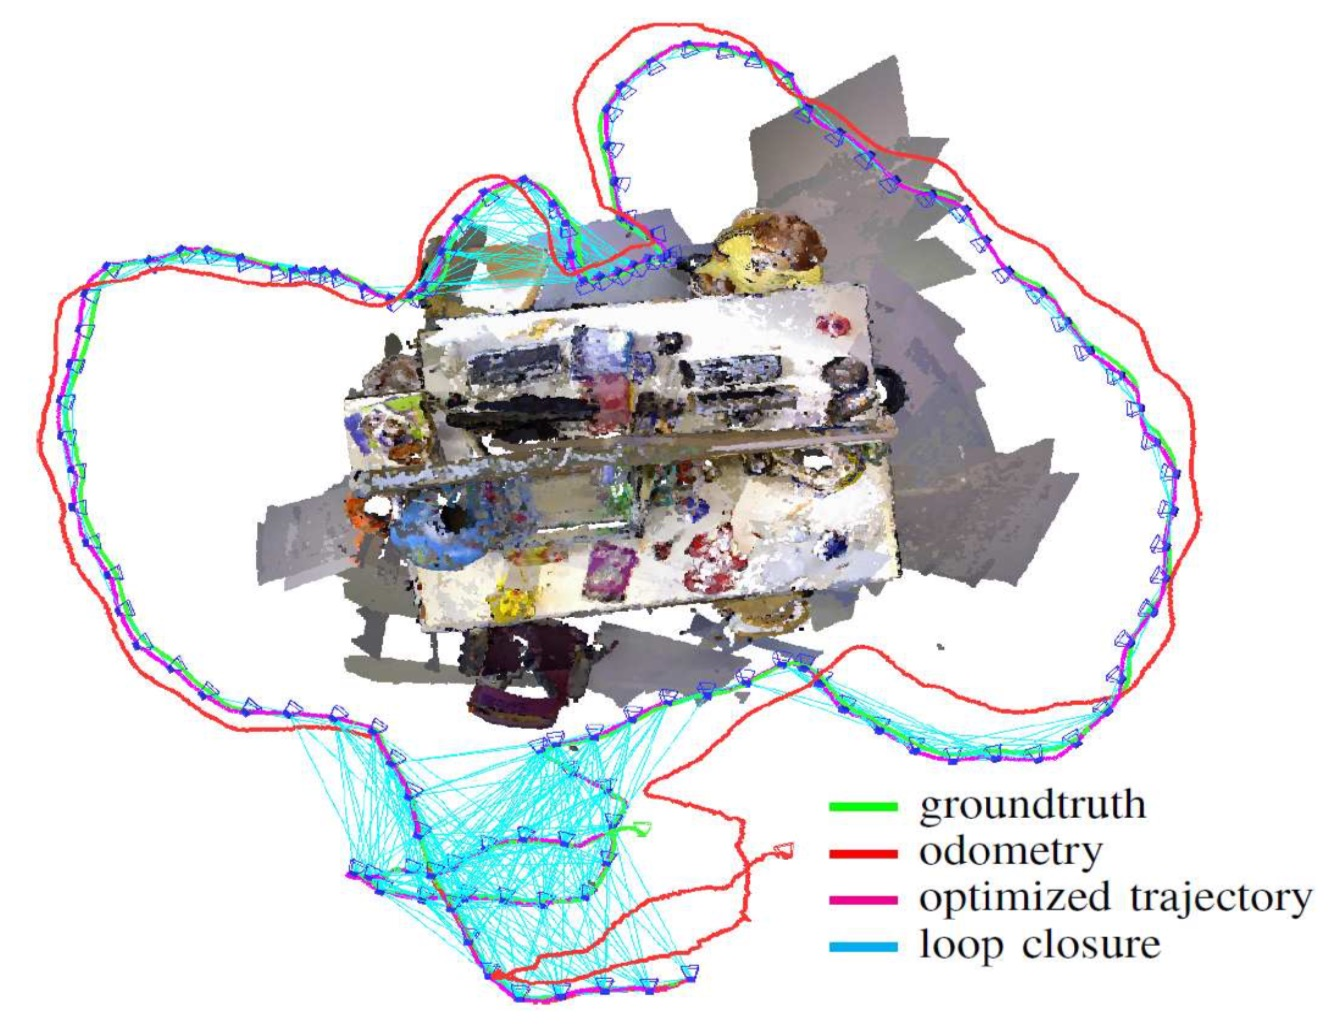
\includegraphics[width=0.9\linewidth]{Images/Loop_closure.jpg}
\end{myfigure}

\subsection{Dense Tracking and Mapping}
Newcombe, Lovegrove \& Davison (ICCV 2011) propose an algorithm which computes both the geometry of the scene and the camera motion from a direct and dense algorithm.\\
They compute the inverse depth $u = \frac{1}{h}$ by minimizing a cost function of the form
\begin{equation*}
\begin{split}
    \min_u \sum_{i = 2}^n \int_{\Omega} \left|I_1(x) - I_i \left(\pi g_i \left(\frac{x}{u}\right)\right) \right| \;\mathrm{d}x \\ + \lambda \int_{\Omega} \phi(x) |\nabla u| \;\mathrm{d}x
\end{split}
\end{equation*}
for fixed camera motions $g_i$.
The function $\phi$ introduces an edge-dependent weighting assigning small weights in locations where the input images exhibit strong gradients:
\begin{equation*}
    \phi (x) = \exp(-|\nabla I_{\sigma} (x)|^{\alpha})
\end{equation*}
The camera tracking is then performed with respect to the textured reconstruction in a manner similar to Steinbrücker et al. (2011).
The method is initialized using feature point based stereo.
\begin{myfigure}
 \centering
 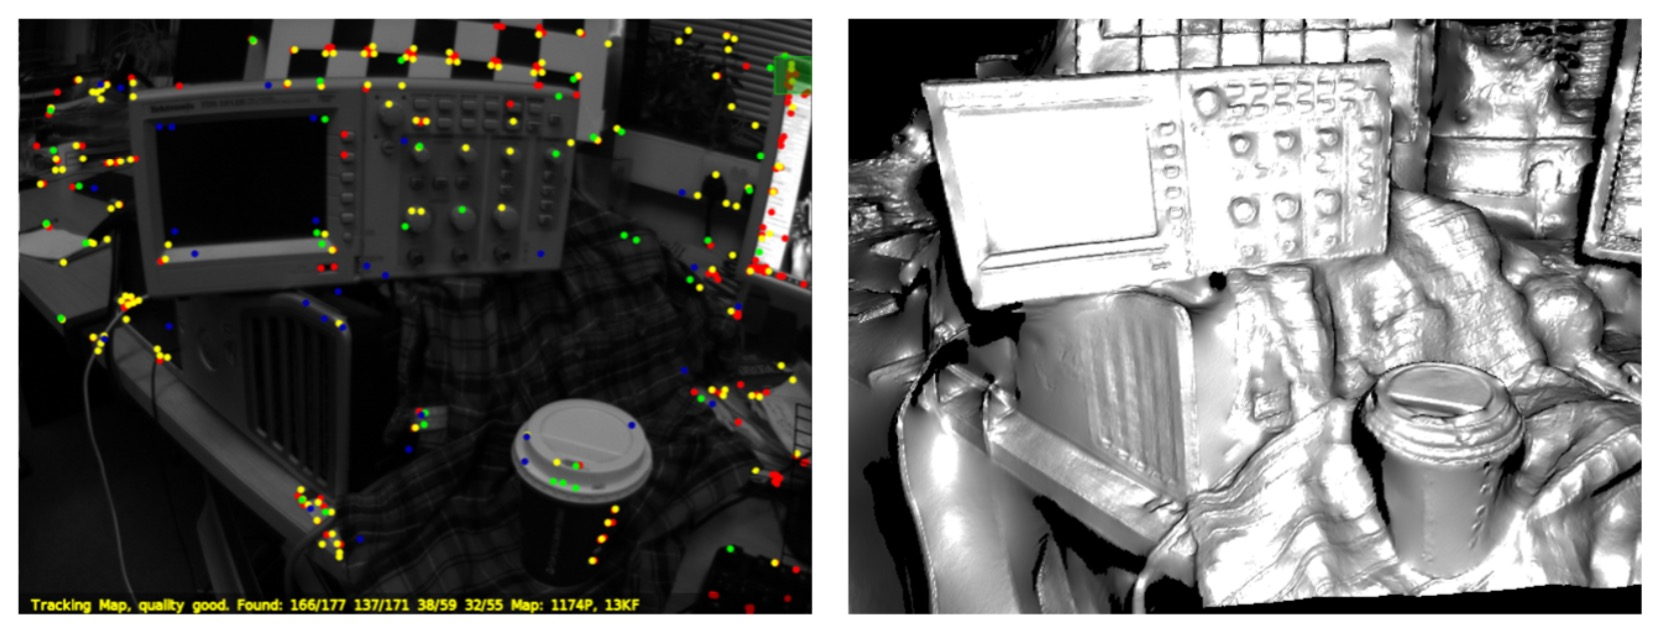
\includegraphics[width=0.9\linewidth]{Images/Dense_tracking_and_mapping.jpg}
\end{myfigure}

\subsection{Large Scale Direct Monocular (LSD) SLAM}
A method for real-time direct monocular SLAM is proposed in Engel, Sturm, Cremers, ICCV 2013 and Engel, Schöps, Cremers, ECCV 2014.
It combines several contributions which make it well-suited for robust large-scale monocular SLAM:
\begin{itemize}
    \item Rather than tracking and putting into correspondence a sparse set of feature points, the method estimates a semi-dense depth map which associates an inverse depth with each pixel that exhibits sufficient gray value variation.
    \item To account for noise and uncertainty each inverse depth value is associated with an uncertainty which is propagated and updated over time like in a Kalman filter.
    \item Since monocular SLAM is invariably defined up to scale only, we explicitly facilitate scaling of the reconstruction by modelling the camera motion using the Lie group of 3D similarity transformations Sim(3).
    \item Global consistency is assured by loop closuring on Sim(3).
\end{itemize}

\paragraph{Tracking by Sim(3) image alignment:}\mbox{}\\
Since reconstructions from a monocular camera are only defined up to scale, Engel, Schöps, Cremers, ECCV 2014 account for rescaling of the environment by representing the camera motion as an element in the Lie group of 3D similarity transformations Sim(3) which is defined as:
\begin{equation*}
\begin{split}
    Sim(3) = \left\{\begin{pmatrix}sR & T\\ 0 & 1 \end{pmatrix} \right. \\ \left. \text{with } R \in SO(3), T \in \mathbb{R}^3, s \in \mathbb{R_{+}}\right\}
\end{split}
\end{equation*}
One can minimize a nonlinear least squares problem
\begin{equation*}
    \min_{\xi \in sim(3)} \sum_i w_i r_i^2 (\xi)
\end{equation*}
where $r_i$ denotes the color residuum across different images and $w_i$ a weighting as suggested in Kerl et al. IROS 2013.
The above cost function can then be optimized by a weighted Gauss-Newton algorithm on the Lie group $Sim(3)$:
\begin{equation*}
\begin{split}
    \xi^{t+1} = \Delta_{\xi} \circ \xi^{(t)} \\ \text{with } \Delta_{\xi} = (J^T W J)^{-1} J^T W r, \quad J = \frac{\partial r}{\partial \xi}
\end{split}
\end{equation*}

Despite its popularity, LSD SLAM has several shortcomings:
\begin{itemize}
\item While the pose graph optimization allows to impose global consistency, it merely performs a joint optimization of the extrinsic parameters associated with all keyframes. In contrast to a full bundle adjustment, it does not optimize the geometry. This is hard to do in realtime, in particular for longer sequences.
\item LSD SLAM actually optimizes two different cost functions for estimating geometry and camera motion.
\item LSD SLAM introduces spatial regularity by a spatial filtering of the inverse depth values. This creates correlations among the geometry parameters which in turn makes Gauss-Newton optimization difficult.
\item LSD SLAM is based on the assumption of brightness constancy. In real-world videos, brightness is often not preserved. Due to varying exposure time, vignette and gamma correction, the brightness can vary substantially. While feature descriptors are often invariant to these changes, the local brightness itself is not.
\end{itemize}

\subsection{Direct Sparse Odometry}
Engel, Koltun, Cremers, PAMI 2018 suggest that brightness variations due to vignette, gamma correction and exposure time can be eliminated by a complete photometric calibration: \begin{equation*}
    I(x)=G \left(t V(x) B(x) \right)
\end{equation*}
where the measured brightness $I$ depends on the irradiance $B$, the vignette $V$, the exposure time $t$ and the camera response function $G$ (gamma function).
$G$ and $V$ can be calibrated beforehand, $t$ can be read out from the camera. \par

\paragraph{Windowed joint optimization:}\mbox{}\\
A complete bundle adjustment over longer sequences is difficult to carry out in real-time because the number of 3D point coordinates may grow very fast over time.
Furthermore new observations are likely to predominantly affect parameters associated with neighboring structures and cameras.
For a given data set, one can study the connectivity graph, i.e. a graph where each node represents an image and two nodes are connected if they look at the same 3D structure.\\
Direct Sparse Odometry therefore reverts to a windowed joint optimization, the idea being that from all 3D coordinates and camera frames only those in a recent time window are included. The remaining ones are marginalized out.\\
If one avoid spatial filtering and selects only a sparser subset of points, then the points can be assumed to be fairly independent.
As a result the Hessian matrix becomes sparser and the Schur complement can be employed to make the Gauss-Newton updates more efficient.

\begin{myfigure}
	\centering
	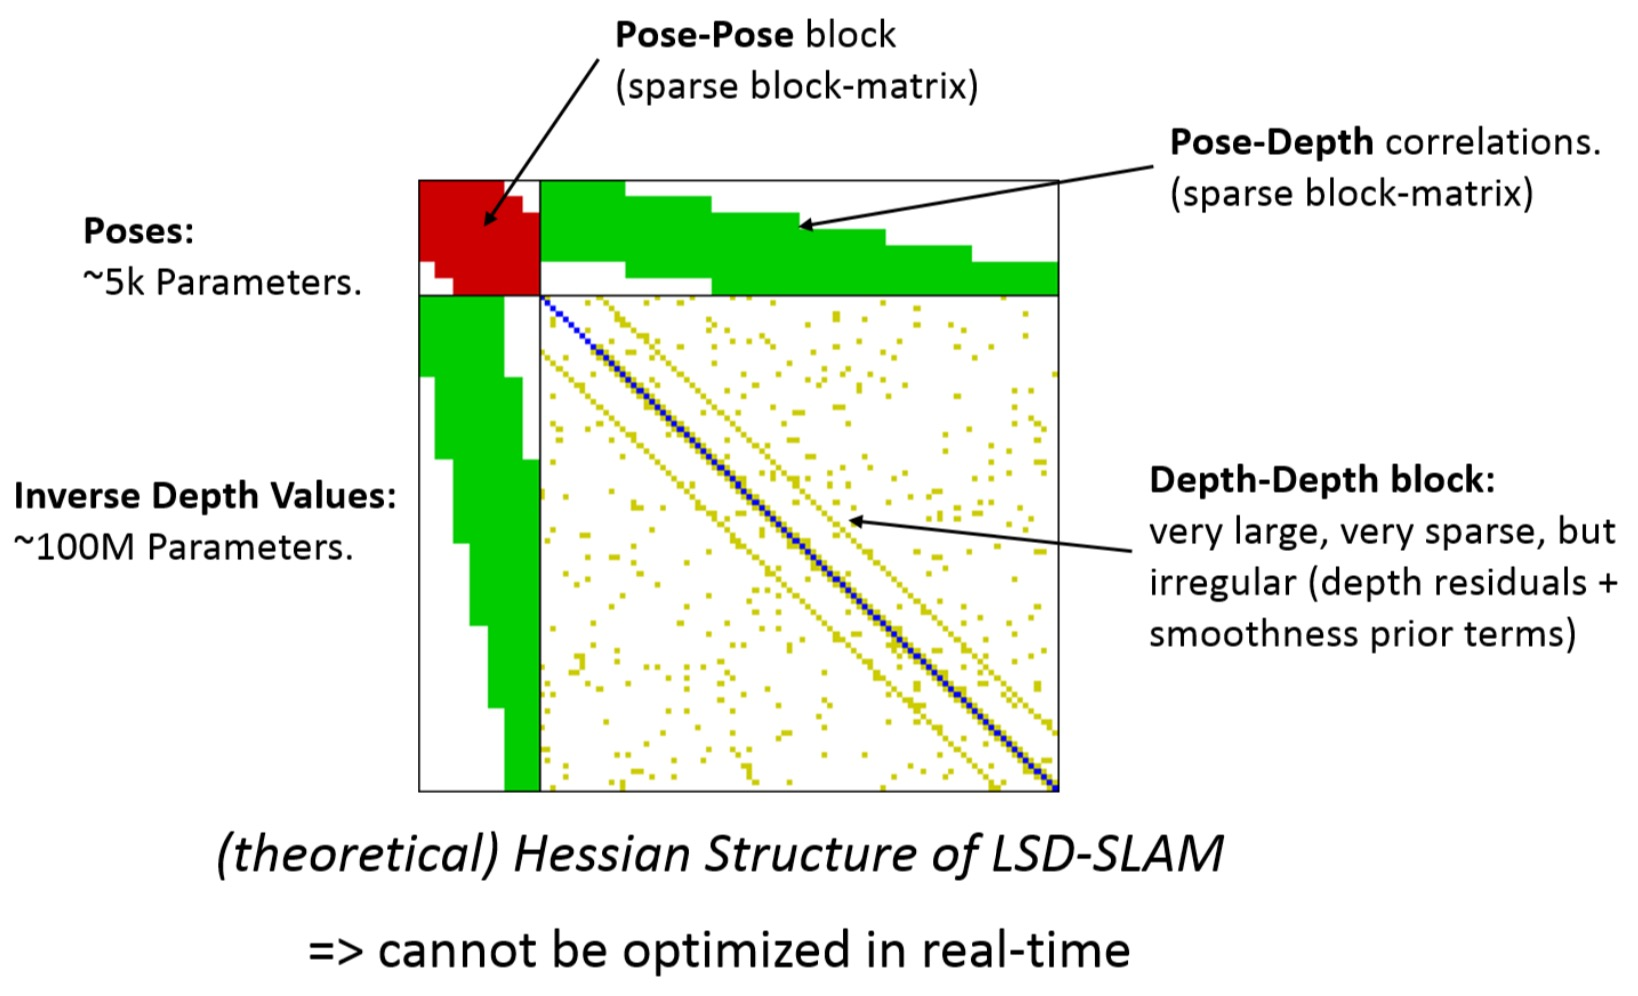
\includegraphics[width=0.9\linewidth]{Images/Direct_Sparse_Odometry.jpg}
	\captionof{figure}{Effect of Spatial Correlation on the Hessian Matrix}
\end{myfigure}

Solving the Newton update step (called normal equation)
\begin{equation*}
    H x = \begin{pmatrix}H_{\alpha \alpha} & H_{\alpha \beta}\\ H_{\alpha \beta} & H_{\beta \beta} \end{pmatrix}
    \begin{pmatrix}x_{\alpha} \\ x_{\beta}\end{pmatrix} = \begin{pmatrix}g_{\alpha} \\ g_{\beta}\end{pmatrix}
\end{equation*}
for the unknowns $x_{\alpha}$ (update in pose parameters) and $x_{\beta}$ (update in depth parameters) is usually done by QR decomposition for large problems.
Here, left-multiplication with the matrix
\begin{equation*}
    \begin{pmatrix}I & -H{\alpha \beta} H_{\beta \beta}^{-1}\\ 0 & I \end{pmatrix}
\end{equation*}
leads to
\begin{equation*}
    \begin{pmatrix}S & 0\\H_{\alpha \beta}^T & H_{\beta \beta} \end{pmatrix} \begin{pmatrix}x_{\alpha} & x_{\beta} \end{pmatrix} = \begin{pmatrix}g_{\alpha} - H_{\alpha \beta} H_{\beta \beta}^{-1} g_{\beta}\\ g_{\beta} \end{pmatrix}
\end{equation*}
where $S = H_{\alpha \alpha} - H_{\alpha \beta} H_{\beta \beta}^{-1} H_{\alpha \beta}^T$ is the Schur complement of $H_{\beta \beta}$ in $H$.
\end{multicols}

\begin{multicols}{2}[\section{Variational Methods: A Short Intro}]
\subsection{Variational Methods}
Variational methods are a class of optimization methods. They are popular because they allow to solve many problems in a mathematically transparent manner. Instead of implementing a heuristic sequence of processing steps (as was commonly done in the 1980's), one clarifies beforehand what properties an optimal solution should have.\\
That does not require extensive training data like for better-performing neural networks.\\
Applications are e.g. spatially dense multiple view reconstruction or motion estimation and optical flow.\\
Variational methods have many advantages over heuristic multi-step approaches (such as the Canny edge detector):
\begin{itemize}
    \item A mathematical analysis of the considered cost function allows to make statements on the existence and uniqueness of solutions.
    \item Approaches with multiple processing steps are difficult to modify. All steps rely on the input from a previous step. Exchanging one module by another typically requires to re-engineer the entire processing pipeline.
    \item Variational methods make all modeling assumptions
    transparent, there are no hidden assumptions.
    \item Variational methods typically have fewer tuning parameters. In addition, the effect of respective parameters is clear.
    \item Variational methods are easily fused – one simply adds respective energies / cost functions.
\end{itemize}

\subsection{Variational Image Smoothing}
Let $f: \Omega \rightarrow \mathbb{R}$ be a grayvalue input image on the domain $\Omega \subset \mathbb{R}^2$. We assume that the observed image arises by some ’true’ image corrupted by additive noise. We are interested in a denoised version u of the input image f. \\
The approximation u should fulfil two properties:
\begin{itemize}
    \item It should be as similar as possible to f
    \item It should be spatially smooth (i.e. ’noise-free’)
\end{itemize}
Both of these criteria can be entered in a cost function of the
form

\begin{equation*}
    \begin{split}
    E(u) = E_{Data}(u,f) + E_{Smoothness}(u) \quad \\ 
    \text{with} \quad E_{data}(u,f) = \int_{\Omega} (u(x)-f(x))^2 dx \\ 
    \text{and} \quad \int_{\Omega} | \nabla u(x) | ^2 dx
    \end{split}
\end{equation*}

\subsection{Euler-Lagrange Equation}
As a necessary condition for minimizers of a functional the associated Euler-Lagrange equation must hold. For a functional of the form
\begin{equation*}
    E(u) = \int \mathcal{L} (u, u') dx
\end{equation*}
it is given by 
\begin{equation*}
    \frac{dE}{du} = \frac{\partial \mathcal{L}}{\partial u} - \frac{d}{dx} \frac{\partial \mathcal{L}}{\partial u'} = 0
\end{equation*}
\begin{itemize}
    \item The central idea of variational methods is therefore to determine solutions of the Euler-Lagrange equation of a given functional. For general non-convex functionals this is a difficult problem.
    \item Another solution is to start with an (appropriate) function $u_0(x)$ and to modify it step by step such that in each iteration the value of the functional is decreased. Such methods are called descent methods.
\end{itemize}

For the class of functionals considered above, the gradient
descent is given by the following partial differential equation:
\begin{myfigure}
 \centering
 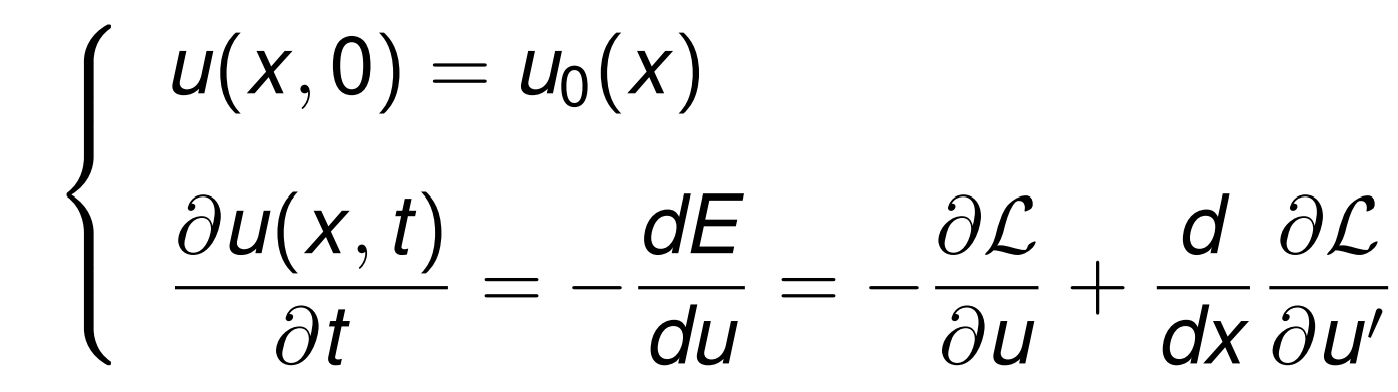
\includegraphics[width=0.7\linewidth]{Images/graddes.png}
\end{myfigure}

If the gradient descent evolution converges: $\partial u / \partial t = - dE / du = 0$
then we have found a solution for the Euler-Lagrange equation.

\section{Variational Multiview Reconstruction }
Shape optimization is a field of mathematics that is focused on formulating the estimation of geometric structures by means of optimization methods.
There exist numerous representations of shape which can loosely be grouped into two classes:
\begin{itemize}
    \item Explicit representations: The points of a surface are represented explicitly (directly), either as a set of points, a polyhedron or a parameterized surface.
    \item Implicit representations: The surface is represented implicity by specifying the parts of ambient space that are inside and outside a given surface.
\end{itemize}
\subsection{Explicit vs. Implicit Representations}
\begin{itemize}
    \item Implicit representations typically require more memory in order to represent a geometric structure at a specific resolution. Rather than storing a few points along the curve or surface, one needs to store an occupancy value for each volume element.
    \item Moving or updating an implicit representation is typically slower
    \item Methods based on implicit representations do not depend on a choice of parametrization
    \item Implicit representations allow to represent objects of arbitrary topology
    \item can be formulated as convex optimization problems and can then be optimized globally
\end{itemize}

\subsection{Multiview Reconstruction}
If the voxel $x \in V$ of the given volume $V \subset \mathbb{R}^3$ was on the surface then (up to visibility issues) the projection of that voxel into each image should give rise to the same color (or local texture). Thus we can assign to each voxel $x \in V$ a so-called photoconsistency function $\rho : V \rightarrow [0,1] $ which takes on low values (near 0) if the projected voxels give rise to the same color (or local texture) and high values (near
1) otherwise.

The reconstruction from multiple views can now be formulated
as finding the maximally photoconsistent surface, i.e. a surface
$S_{opt}$ with an overall minimal photoconsistency score:
\begin{equation*}
    s_{opt} = \arg \min_S \int_S \rho (s) ds
\end{equation*}
Formulated as a convex, constrained optimization problem:

\begin{myfigure}
 \centering
 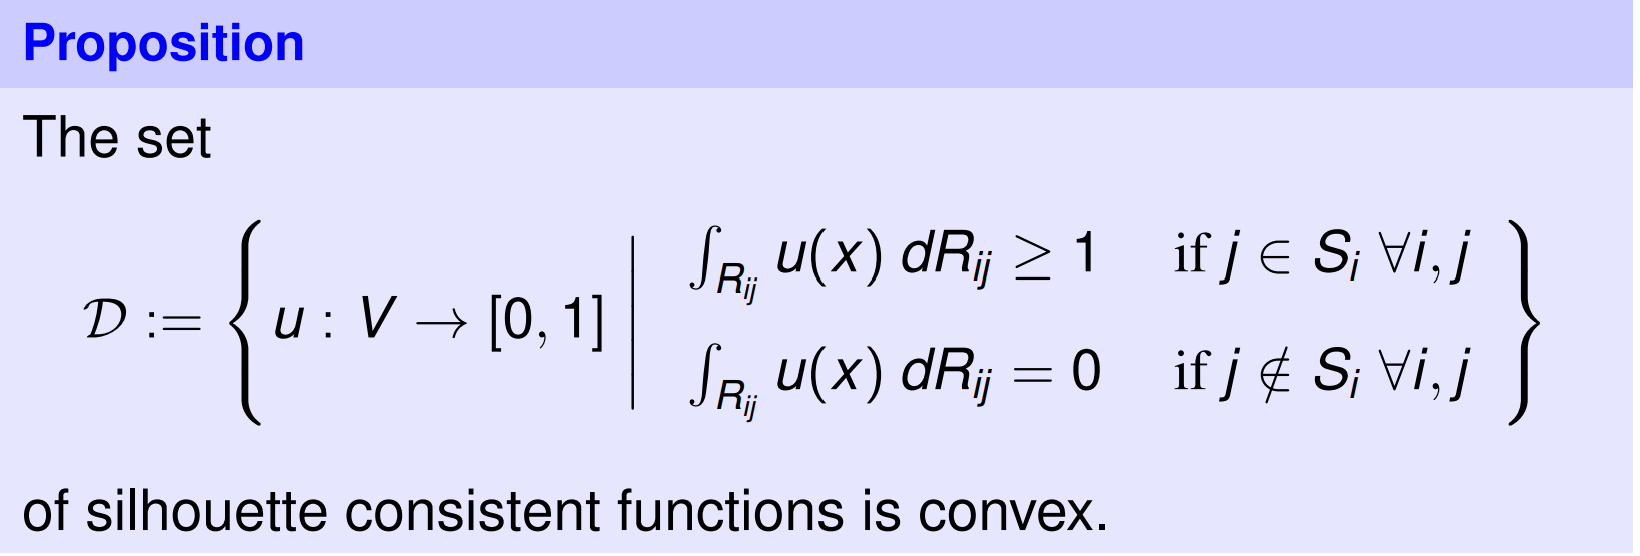
\includegraphics[width=1\linewidth]{Images/prop.png}
\end{myfigure}

\begin{myfigure}
 \centering
 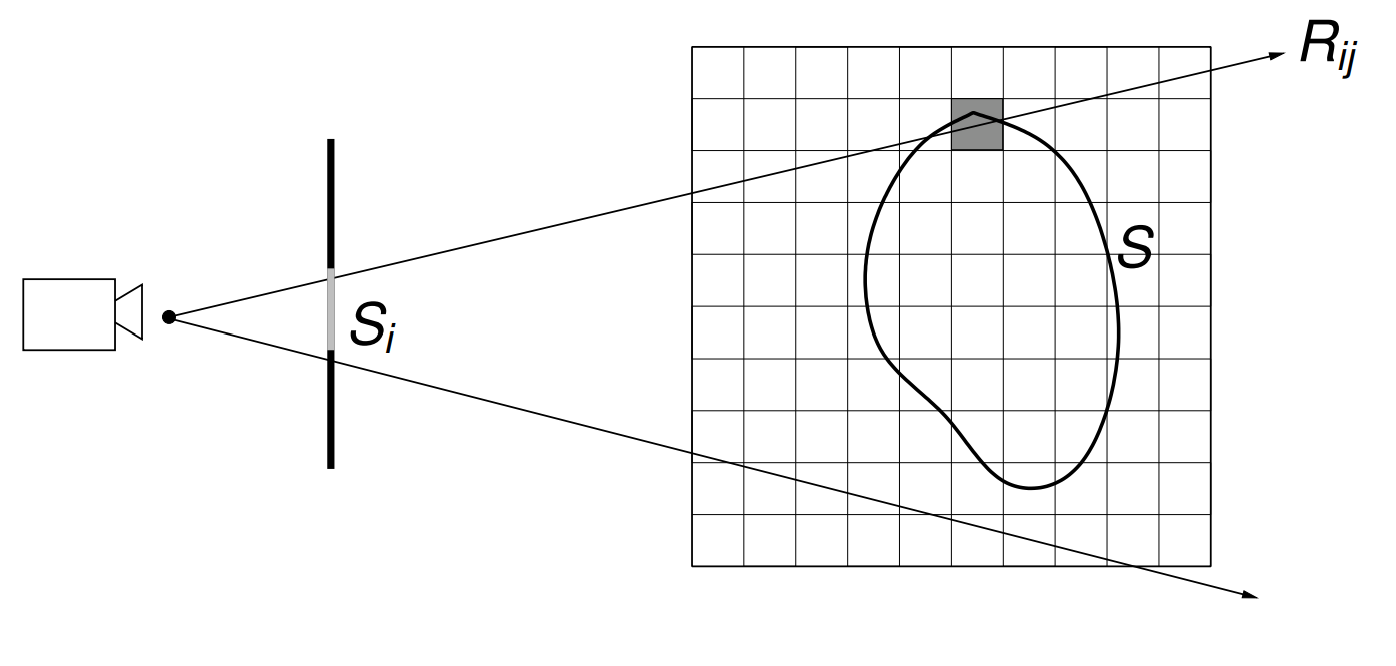
\includegraphics[width=1\linewidth]{Images/cam.png}
\end{myfigure}

\subsection{Multiview Texture Reconstruction}
In addition to the dense geometry S, we can also recover the texture $T: S \rightarrow \mathbb{R}^3$ of the object from the images $\mathcal{I}_i : \Omega_i \rightarrow \mathbb{R}^3$:
\begin{equation*}
    \min_{T:S \rightarrow \mathbb{R}^3} \sum_{i=1}^{n} \int_{\Omega_i} (b * (T \circ \pi_i^{-1})- \mathcal{I}_i)^2 dx + \lambda \int_S || \nabla_s T|| ds
\end{equation*}

\end{multicols}

\clearpage
\appendix

\section{Special Matrices and Properties}
\begin{description}
     \item[symmetric matrices] $A^T = A \\ \Rightarrow \ \langle Ax, y \rangle =  \langle x, Ay \rangle \text{ and eigenvectors } \langle v_i, v_j \rangle = 0, \quad i \neq j
     \\ \Rightarrow$ all eigenvalues are real
     \item[skew-symmetric/antisymmetric matrices] $A^T = -A \\ \Rightarrow \ \begin{pmatrix}0 & -a_3 & a_2\\ a_3 & 0 & -a_1\\ -a_2 & a_1 & 0\end{pmatrix} \cdot b = a \times b \quad a, b \in \mathbb{R}^3 \\
     \Rightarrow$ all eigenvalues are zero or imaginary
     \item[orthogonal matrices] $Q^T = Q^{-1} \\ \Rightarrow \ \text{eigenvectors form a basis} \\ \Rightarrow \ QQ^T = Q^T Q = I$
     \item[inverse 2x2 matrices] $A = \begin{pmatrix} a & b \\ c & d \end{pmatrix} \rightarrow A^{-1} = \frac{1}{ad-bc} \begin{pmatrix} d & -b \\ -c & a \end{pmatrix}$
     \item[singular matrices] $\det(A) = 0 \\ \Rightarrow \ A \text{ not invertible}$
     \item[diagonal matrices] all entries but the main diagonal are zero   
     \item[positive-definite] $\lambda_1, \dots ,\lambda_n > 0 \\ \Rightarrow \ x^T A x > 0 \quad x \neq \vec{0}$
     \item[positive-semidefinite] $\lambda_1, \dots ,\lambda_n \geq 0$
     \item[negative-definite] $\lambda_1, \dots ,\lambda_n < 0$
     \item[indefinite] $-\infty < \lambda_1, \dots ,\lambda_n < \infty$
     \item[Properties of determinants] $A,B \in \mathbb{R}^{n \times n}$
     \begin{flalign*}
     	\det\begin{pmatrix} a & b \\ c & d \end{pmatrix} &= ad - bc\\
     	\det(AB) &= \det(A) \cdot \det(B)\\
     	\det(A^{-1}) &= \frac{1}{\det(A)}\\
     	\det(A^T) &= \det(A)\\
     	\det(kA) &= k^n \det(A), k \in \mathbb{R}\\
     	\det(A) &= \lambda_1 \cdot ... \cdot \lambda_n
     \end{flalign*}
\end{description}

\section{Rotation Matrices in SO(3)}\label{section:rotation_matrices}
Rotation around x-axis:
\begin{equation*}
    R_x (\alpha) =\begin{pmatrix}1 & 0 & 0\\
    0 & \cos \alpha & -\sin \alpha\\ 0 & \sin \alpha & \cos \alpha \end{pmatrix}
\end{equation*}

Rotation around y-axis:
\begin{equation*}
    R_y (\alpha) =\begin{pmatrix}\cos \alpha & 0 & \sin \alpha\\
    0 & 1 & 0\\ -\sin \alpha & 0 & \cos \alpha \end{pmatrix}
\end{equation*}

Rotation around z-axis:
\begin{equation*}
    R_z (\alpha) =\begin{pmatrix}\cos \alpha & -\sin \alpha & 0\\
    \sin \alpha & \cos \alpha & 0\\ 0 & 0 & 1 \end{pmatrix}
\end{equation*}

\section{Convolution}
\begin{equation*}
    (f * g)(x) = \int_{\mathbb{R}^n} f(\tau) \ g(x-\tau) \;\mathrm{d}\tau
\end{equation*}

\end{document}
